
\documentclass[11pt,a4paper]{article}
\usepackage[margin=2.2cm]{geometry}
\usepackage[T1]{fontenc}
\usepackage{setspace}
\usepackage{booktabs}
\usepackage{graphicx}
\graphicspath{{../}{../figures/}}
\usepackage{caption}
\usepackage{amsmath,amssymb}
\usepackage[round,authoryear]{natbib}
\usepackage{float}
\usepackage{enumitem}
\usepackage{fancyhdr}
\usepackage[hidelinks]{hyperref}
\usepackage{titlesec}
\usepackage{xcolor}

\setstretch{1.0}
\setlength{\parindent}{0pt}
\setlength{\parskip}{1pt}
\captionsetup{font=small,labelfont=bf,skip=3pt}
\setlength{\textfloatsep}{8pt plus 2pt minus 2pt}
\setlength{\floatsep}{8pt plus 2pt minus 2pt}
\setlength{\intextsep}{8pt plus 2pt minus 2pt}
\renewcommand{\arraystretch}{0.95}
\setlength{\tabcolsep}{4pt}
\setlength{\emergencystretch}{2em}
\captionsetup[table]{position=top}
\pagestyle{fancy}
\fancyhf{}
\fancyhead[L]{\footnotesize DSA5205 Project 2}
\fancyhead[R]{\footnotesize Ridge-based cross-sectional equity strategy}
\fancyfoot[C]{\thepage}
\renewcommand{\headrulewidth}{0.4pt}
\titleformat{\section}{\large\bfseries}{\thesection}{0.6em}{}
\titleformat{\subsection}{\normalsize\bfseries}{\thesubsection}{0.5em}{}
\titlespacing*{\section}{0pt}{2.0ex plus 0.5ex}{1.0ex}
\titlespacing*{\subsection}{0pt}{1.5ex plus 0.4ex}{0.8ex}
\newcommand{\team}{Group X}
\begin{document}

\begin{titlepage}
\centering
\vspace*{1.4cm}
{\small DSA5205 --- Data Science for Quantitative Finance\par}
\vspace{0.4cm}
{\small Project 2: Design, Validate, and Analyze an Original Asset Trading Strategy\par}
\vspace{2.2cm}
{\LARGE\bfseries Ridge Regression for Cross-Sectional Equity Selection\par}
\vspace{0.6cm}
{\Large A Validation and Out-of-Sample Study of a Momentum--Volatility Screened Portfolio\par}
\vspace{2.2cm}
{\large DSA5205 Project 2 Team\par}
\vspace{1.4cm}
{\normalsize 11 November 2026\par}
\vfill
\begin{minipage}{0.86\textwidth}
\small
\textbf{Scope.} This report studies one primary Ridge-based strategy, compares it with three alternative machine-learning models, two momentum baselines and two investable ETFs, and reports the results of a chronological out-of-sample evaluation. The original exploratory Ridge extension is retained as exploratory analysis. All results are for academic research and historical backtesting only.
\end{minipage}
\vspace{1.2cm}
\end{titlepage}
\begin{abstract}

This paper studies whether Ridge Regression, trained on economically motivated financial predictors, can generate useful cross-sectional stock rankings for a systematic US equity portfolio. The primary strategy screens a liquid universe with a momentum--volatility double sort, ranks the resulting thirty candidates with Ridge, buys the ten highest predicted returns at equal weights, rebalances monthly, and executes at the next open net of 20 basis points per traded side. Ridge is designated as the primary research model on economic and diagnostic grounds: its L2 penalty is appropriate for a dense set of correlated predictors, it produces the highest validation rank information coefficient of the four models, and rolling-window diagnostics show lower relative coefficient movement than LASSO. LASSO, Random Forest and XGBoost are evaluated as alternative forecasting models on an identical prediction task, while B1, B3, SPY and QQQ provide momentum baselines and investable benchmarks. Training uses 2010--2019, validation 2020--2021, and the final holdout is 2022--2025. Ridge earns a 43.0\% net compound annual return with a 1.27 Sharpe ratio and a -28.5\% maximum drawdown over the holdout, comfortably ahead of SPY (12.7\%, 0.86) and QQQ (14.8\%, 0.80). It does not beat simple momentum: B1 earns 73.1\% with a 1.66 Sharpe and a -19.2\% drawdown, and B3 earns 51.5\% with a 1.59 Sharpe and a -15.0\% drawdown. Within the same candidate pool, the Ridge ranking underperforms a momentum ranking by 8.5 percentage points of annual return and 0.32 of Sharpe, with higher turnover. The evidence therefore supports Ridge as an economically defensible forecasting model that adds value relative to passive benchmarks, but not as a source of incremental value over momentum-based selection in this sample. The paper documents the full validation and out-of-sample process, identifies the earlier automatic LASSO rule as a superseded auxiliary artifact, and discloses that the Ridge designation is not a clean pre-registration because the project history includes prior out-of-sample review.

\end{abstract}

\section{Introduction and Research Motivation}

\subsection{Systematic cross-sectional equity selection}

Systematic equity strategies replace discretionary stock picking with a reproducible rule that maps observable firm characteristics into portfolio positions. The appeal is not that the rule is always right, but that it can be specified before the data are seen, evaluated on a held-out period, and audited afterwards. The academic literature has documented many cross-sectional regularities, including short-term reversal \citep{jegadeesh1990}, momentum \citep{jegadeesh1993}, value and momentum jointly \citep{asness2013}, and a long list of firm characteristics whose individual predictive power is small and unstable \citep{hou2020, feng2020}. Machine-learning methods are attractive in this setting because they can combine many weak, correlated predictors, but they also increase the risk of fitting noise \citep{gu2020}.

This paper takes a deliberately narrow version of that problem. The universe is a liquid subset of the S\&P 500. The candidate pool is formed by a transparent momentum--volatility double sort. The forecasting model ranks thirty names, and the portfolio holds the top ten at equal weights. Almost all of the complexity is in the forecast; the portfolio layer is intentionally simple. That design makes the research question sharp: does the forecasting model produce a better ordering of the candidates than simpler alternatives?

\subsection{Research question and contributions}

The primary research question is whether Ridge Regression, trained on economically motivated financial predictors, can generate useful cross-sectional stock rankings and improve the performance of a systematic equity portfolio relative to simpler investment alternatives.

The paper makes four contributions. First, it evaluates Ridge against three materially different forecasting algorithms---LASSO, Random Forest and XGBoost---on exactly the same universe, features, target, split, trading rule and cost assumption. The comparison therefore isolates the forecasting algorithm rather than confounding it with strategy design. Second, it grounds the Ridge choice in the correlation structure of the predictors and in rolling coefficient-stability diagnostics, rather than in a single validation metric. Third, it reports the primary strategy against two momentum baselines and two investable ETFs on a common out-of-sample window, and it verifies that the two backtest engines used to produce those series agree on dates, benchmark returns and the B3 selection rule. Fourth, it is explicit about what the evidence does \emph{not} show: in this sample, the Ridge ranking does not improve on a simple momentum ranking within the same candidate pool.

\subsection{Relation to the literature}

The forecasting exercise is related to the empirical asset-pricing literature that treats expected returns as a function of many characteristics \citep{gu2020, kelly2019, freyberger2020}. The regularisation choice is the classical ridge-versus-lasso question \citep{hoerl1970, tibshirani1996}: ridge shrinks a dense coefficient vector, while lasso selects a sparse one. The portfolio evidence is related to the momentum literature \citep{jegadeesh1993, asness2013, moskowitz2012} and to the broader critique that many published anomalies weaken out of sample \citep{mclean2016, hou2020}. The project does not attempt a structural model of returns; it asks whether a specific, pre-specified forecasting rule is useful for a specific portfolio construction.

The remainder of the paper is organised as follows. Section~\ref{sec:markets} describes the market, assets and timing. Section~\ref{sec:data} defines labels and features. Section~\ref{sec:benchmarks} defines the benchmarks. Section~\ref{sec:model} presents the Ridge rationale and the correlation and stability diagnostics. Section~\ref{sec:split} documents the chronological split. Section~\ref{sec:training} describes training, and Section~\ref{sec:validation} the validation and model-selection policy. Section~\ref{sec:trading} states the trading rules and costs. Section~\ref{sec:oos} reports the out-of-sample evidence. Section~\ref{sec:interpretation} interprets it, Section~\ref{sec:extensions} discusses exploratory extensions, Section~\ref{sec:limitations} lists limitations, and Section~\ref{sec:conclusion} concludes. Section~\ref{sec:reproducibility} documents reproducibility and AI use.


\section{Markets, Assets and Trading Timing}
\label{sec:markets}

\subsection{Market, universe and frequency}

The market is US large-capitalisation equity, traded in US dollars on the NYSE and Nasdaq calendars. The eligible universe is built from the current S\&P 500 constituent list. At each month-end, a stock is eligible if its close is at least \$5, its twenty-day average dollar volume is at least \$10 million, and it has at least 95\% price coverage over the 21-, 63- and 252-session windows. The three hundred most liquid eligible names form the liquid universe. The 300-name cap is a fixed design choice, not a parameter chosen on the test period: it keeps the universe tradable, reduces exposure to illiquid names, provides enough cross-sectional breadth for a 3$\times$3 sort, and makes candidate construction consistent across months. In this data snapshot every month reached the cap, but the rule does not guarantee it; a month with fewer than 90 eligible names is skipped rather than padded.

The strategy trades monthly. Decisions are made after the close of the last trading session of each calendar month, and trades are executed at the open of the next observed session. The holding period therefore runs from one monthly execution open to the next. No intraday information enters the decision, and no same-close execution is assumed.

\subsection{The 3$\times$3 screen and the 3--4--3 allocation}

The screen is a dependent double sort, implemented in the preserved pipeline. Eligible stocks are first ranked by twelve-month momentum (\texttt{mom\_2\_12}) in descending order and split into three approximately equal momentum groups: high, medium and low. Within each momentum group, stocks are sorted by sixty-three-day volatility (\texttt{vol\_63}) in ascending order and split into three approximately equal volatility cells: low, medium and high. Each cell then contributes a fixed number of candidates: three from the low-volatility cell, four from the medium-volatility cell and three from the high-volatility cell. Each momentum group therefore contributes ten names, and the screen produces thirty candidates.

The within-cell ranking depends on the momentum group. The high-momentum group takes the highest \texttt{mom\_2\_12} names in the cell, the low-momentum group takes the lowest, and the medium-momentum group takes the names closest to the cell median. Ties are broken by ticker in ascending order. If a cell contains fewer names than required, the decision date is skipped rather than filled with names outside the cell.

The 3--4--3 allocation is symmetric because ten candidates cannot be divided evenly into three volatility cells. Assigning the additional candidate to the middle cell avoids favouring either volatility extreme. It is a fixed, interpretable design choice; the paper does not claim that 3--4--3 is empirically optimal or that medium-volatility stocks are superior. The screen is risk-characteristic-aware, but it does not minimise portfolio variance and it does not guarantee that the final ten holdings are diversified across volatility groups. Candidate-universe diversification is not the same as final-portfolio diversification.

\subsection{Assets, benchmarks and currency}

The tradable instruments in the backtest are the individual stocks in the candidate pool, plus SPY and QQQ as buy-and-hold benchmarks. The base currency is the US dollar; no FX conversion is required. SPY tracks the S\&P 500 and QQQ tracks the Nasdaq-100. Both are liquid, investable ETFs and are therefore genuine alternatives for a real investor, unlike the momentum baselines, which are systematic rules rather than products.

\subsection{Data sources and corporate actions}

Prices, volumes, dividends and splits are obtained from Yahoo Finance through the \texttt{yfinance} interface. The constituent list is the current membership table published on Wikipedia. Adjusted prices reflect dividends and splits; the backtest uses adjusted opens for both entry and exit, so the return series is total-return in nature. The data snapshot is frozen for reproducibility.

Adjusted opens are used consistently for both entry and exit, so dividends and splits are reflected in every label and backtest return. The treatment is not a manual corporate-action reconstruction: vendor adjusted prices can also embed spin-off or special-distribution adjustments that are not recorded in the split field, so adjusted returns can differ from raw-price returns around such events. This is a documented data limitation, not a correction applied inside the backtest. A verification check on the raw snapshot confirms that there are no non-positive or duplicate observations and that adjusted prices are used consistently. First, using current S\&P 500 constituents to construct the historical equity universe introduces potential survivorship and constituent-selection bias into the active stock-selection strategies: firms that were removed from the index are absent, and current survivors are over-represented. This may overstate their historical performance relative to SPY and QQQ, whose buy-and-hold returns are calculated directly from historical ETF prices. Second, vendor price adjustments and corporate-action treatment may affect both individual-stock histories and ETF return calculations, and Yahoo Finance is not an exchange-grade point-in-time database. Neither limitation is resolved by the modelling choices, and the direction or magnitude of the survivorship effect is not precisely measured here.

\subsection{The eight evaluated strategies}

Table~\ref{tab:strategies} lists the eight strategies. The four machine-learning strategies share the same thirty-candidate pool, features, target, split, execution and cost assumptions; only the forecasting algorithm differs. B1 and B3 are momentum baselines. B1 selects the momentum Top 10 from the full liquid universe, while B3 selects the momentum Top 10 within the same thirty-candidate pool used by the ML models. SPY and QQQ are investable buy-and-hold benchmarks.

The distinction between a trading baseline and an investable benchmark matters. A baseline answers ``does the model add value relative to a simple systematic rule?''. An investable benchmark answers ``would an investor have been better off in an index ETF?''. The paper reports both because the answers differ.

\begin{table}[H]
\centering
\footnotesize
\begin{tabular}{p{2.2cm}p{3.4cm}p{5.8cm}p{2.6cm}}
\toprule
Strategy & Role in the study & Selection rule & Weighting \\
\midrule
Ridge & Primary model & 3$\times$3 pool, Ridge Top 10 & Equal 10\% \\
LASSO & Alternative ML & 3$\times$3 pool, LASSO Top 10 & Equal 10\% \\
Random Forest & Alternative ML & 3$\times$3 pool, RF Top 10 & Equal 10\% \\
XGBoost & Alternative ML & 3$\times$3 pool, XGB Top 10 & Equal 10\% \\
B1 & Momentum baseline & Momentum Top 10, full liquid universe & Equal 10\% \\
B3 & Momentum baseline & Momentum Top 10, 3$\times$3 pool & Equal 10\% \\
SPY & Investable benchmark & Buy-and-hold S\&P 500 ETF & Fully invested \\
QQQ & Investable benchmark & Buy-and-hold Nasdaq-100 ETF & Fully invested \\
\bottomrule
\end{tabular}
\caption{Strategy roles. B1 and B3 are systematic trading baselines, not investable index products; SPY and QQQ are investable buy-and-hold alternatives.}
\label{tab:strategies}
\end{table}



\section{Labels, Features and Data Preparation}
\label{sec:data}

\subsection{Prediction target and horizon}

The target is the next holding-period simple return computed from adjusted opens:
\begin{equation}
y_t=\frac{P^{\text{adj open}}_{t+H}}{P^{\text{adj open}}_{t}}-1,
\label{eq:target}
\end{equation}
where $t$ is the execution open after the decision date and $t+H$ is the execution open after the next rebalance. For monthly rebalancing, $H$ is approximately one month. Using adjusted opens rather than closes ensures that the label matches the price at which a position could actually be established and unwound, and that dividends and splits are reflected.

The timing convention is strict: \texttt{decision\_date} $<$ \texttt{execution\_date} $<$ \texttt{label\_end\_date} for every observation. The model at date $t$ uses features computed from data up to the decision close and predicts a return that is realised only after the position is opened. Section~\ref{sec:split} describes the additional embargo that prevents labels which settle after a split boundary from entering the earlier stage.

\subsection{The fifteen features}

Table~\ref{tab:features} lists the fifteen features, grouped into five economic categories: momentum, volatility and risk, technical trend, liquidity and trading activity, and price range. All inputs are available at the decision close and none uses future information.

\begin{table}[H]
\centering
\footnotesize
\begin{tabular}{p{2.1cm}p{2.8cm}p{5.3cm}p{3.9cm}}
\toprule
Group & Feature & Definition and lookback & Interpretation \\
\midrule
Momentum & mom\_21 & 21-session total return & Short-horizon continuation or reversal \\
Momentum & mom\_63 & 63-session total return & Quarterly momentum \\
Momentum & mom\_126 & 126-session total return & Semi-annual momentum \\
Momentum & mom\_2\_12 & 12-month return, skipping the last month & Classic 12--1 momentum \\
Momentum & relative\_mom\_63 & 63-session return minus SPY return & Relative strength \\
Volatility/risk & vol\_21 & Annualised 21-session realised volatility & Short-term risk \\
Volatility/risk & vol\_63 & Annualised 63-session realised volatility & Screening volatility \\
Volatility/risk & beta\_252 & 252-session rolling beta to SPY & Systematic exposure \\
Volatility/risk & drawdown\_63 & Price relative to 63-session high & Recent loss state \\
Trend & ma\_ratio\_50 & Price relative to 50-session moving average & Short-term trend \\
Trend & ma\_ratio\_200 & Price relative to 200-session moving average & Long-term trend \\
Trend & rsi\_14 & 14-session relative strength index & Overbought/oversold \\
Liquidity & ln\_adv\_20 & Log 20-session average dollar volume & Size and liquidity \\
Liquidity & volume\_ratio\_21 & Volume relative to 21-session average & Abnormal activity \\
Range & range\_hl & High--low range scaled by close & Intraday price pressure \\
\bottomrule
\end{tabular}
\caption{The fifteen predictors, grouped by economic mechanism. All inputs are available at the month-end decision close.}
\label{tab:features}
\end{table}


The feature set is compact and interpretable rather than empirically optimal. Fifteen characteristics keep the parameter-to-observation ratio manageable in a sample of a few thousand candidate-months and allow the coefficients to be read economically. No claim is made that fifteen is the best possible number, and the paper does not search over feature subsets.

\subsection{Why multiple horizons}

Momentum is measured at 21, 63, 126 and 12--1 months, and trend is measured with 50- and 200-session moving-average ratios. These horizons are not redundant even when they are correlated. Short horizons are more sensitive to reversal and microstructure effects, while twelve-month momentum captures slower fundamental trends. The 12--1 construction deliberately skips the most recent month, following the momentum literature, to reduce contamination from short-term reversal \citep{jegadeesh1993}. Relative momentum subtracts the SPY return over the same window, so it measures cross-sectional strength rather than market direction.

The volatility block separates short- and medium-horizon realised volatility, market beta and recent drawdown. The trend block captures whether the price is above or below its moving averages and whether it is overbought or oversold. The liquidity block captures size and abnormal trading activity. The range feature captures intraday price pressure. Together they represent the main mechanisms through which past prices could predict future cross-sectional returns.

\subsection{Cleaning, missing values and outliers}

The data pipeline requires finite feature values for every candidate at the decision date. It does not fabricate pre-IPO or post-delisting prices, and it does not globally forward-fill prices. Auxiliary machine-learning features may be carried forward for at most two sessions, but the screening variables---twelve-month momentum, sixty-three-day volatility and log dollar volume---are never forward-filled. Extreme values are not winsorised. The model relies on regularisation and on the screening filters, which require a minimum price and liquidity. This choice is transparent but not innocuous: a small number of extreme momentum realisations can influence the fitted coefficients, and a winsorised alternative could produce different results.

\subsection{Scaling and leakage prevention}

Ridge and LASSO standardise features inside a scikit-learn \texttt{Pipeline}. The scaler is therefore fitted only on the rows passed to \texttt{fit}, which for training is the 2010--2019 slice and for the final refit is 2010--2021. Validation and test features are transformed with those training parameters. Tree models are scale-invariant and use no scaler. No imputation is performed inside the model.

A row enters training or tuning only if its label has settled by the split boundary. This removes the last two 2019 cohorts from training, because their labels settle in January and February 2020, and the last two 2021 cohorts from validation, because their labels settle in January and February 2022. The test slice is never loaded by the validation or designation stages.


\section{Benchmarks}
\label{sec:benchmarks}

\subsection{Investable benchmarks}

SPY and QQQ are buy-and-hold ETFs. They are charged a single 20 basis point entry cost at the start of the evaluation and no monthly rebalancing cost, because a buy-and-hold investor does not rebalance. This is the correct comparison: applying the active strategy's monthly turnover cost to a passive ETF would overstate the active strategy. Both benchmarks are evaluated on exactly the same decision dates and with the same execution-to-execution return convention as the active strategies.

\subsection{Strategy baselines B1 and B3}

B1 and B3 are systematic momentum rules. B1 ranks the full liquid universe by twelve-month momentum and buys the top ten at equal weights. B3 ranks the thirty candidates produced by the same 3$\times$3 double sort used by the ML strategies and buys the ten highest-momentum names at equal weights. Both execute at the next open and bear the same 20 basis point cost as the active strategies, so their returns are directly comparable.

The two baselines answer different questions. B1 is a complete alternative strategy: it differs from the primary strategy in both the candidate universe and the ranking method. B3 is a cleaner ranking test: it holds the candidate pool, execution and costs fixed and changes only whether the top ten are chosen by momentum or by the model. The Ridge-versus-B3 comparison is therefore the paper's main evidence on whether the forecasting model adds value beyond momentum within the screened pool. The Ridge-versus-B1 comparison is a comparison of complete strategies and cannot be attributed to ranking alone.

\subsection{Why both types of benchmark are needed}

A model that beats SPY but loses to a simple momentum rule has not demonstrated that the model is useful for stock selection; it has demonstrated that equity exposure and a momentum tilt were useful. Conversely, a model that beats momentum but loses to SPY would be difficult to justify to an investor. Reporting both types of benchmark prevents either conclusion from being drawn from a single comparison. The paper also reports turnover and transaction costs for every strategy, because a strategy that earns a higher gross return by trading more intensively may not earn a higher net return.


\section{Model Choice and Overfitting Control}
\label{sec:model}

\subsection{Economic rationale for Ridge}

The fifteen predictors are correlated financial characteristics. Ridge regression estimates a dense linear coefficient vector and penalises its squared Euclidean norm \citep{hoerl1970}:
\begin{equation}
\hat{\beta}_{\text{ridge}}=\arg\min_{\beta}\;\sum_{i=1}^{N}\left(y_i-x_i'\beta\right)^2+\alpha\|\beta\|_2^2 .
\label{eq:ridge}
\end{equation}
The penalty introduces bias but reduces variance, which is valuable when predictors are collinear and the signal-to-noise ratio is low. The resulting score is continuous, which maps naturally into a cross-sectional ranking: the portfolio only needs to know which candidates are likely to be in the top decile, not the precise expected return of every stock.

The economic story is that expected returns depend on several weak, related characteristics and that a shrunk combination of them is more stable than any individual signal. This is a modest claim. It does not require that every feature has independent predictive power, and it does not require that the linear functional form is literally correct. It requires only that the combination is more informative about the ordering of future returns than a single momentum rank.

\subsection{Correlated predictors}

Appendix Figure~\ref{fig:corr} shows the training-period correlation matrix, and Table~\ref{tab:corr} lists the twelve pairs with absolute correlation of at least 0.70. The strongest pair is 63-day momentum and relative 63-day momentum at 0.939, which is mechanical: the two series differ only by the SPY return over the same window. The next strongest pairs link 126-day momentum to the 200-day moving-average ratio (0.936), 21-day momentum to the 50-day moving-average ratio (0.868), and 63-day momentum to the 200-day ratio (0.816). Short and medium volatility are correlated at 0.809.

Correlation does not imply identical economic information. A 63-day and a 126-day return measure different horizons even when they co-move; relative and absolute momentum answer different questions; a moving-average ratio and a trailing return are related but not identical transformations. Removing every correlated feature would discard horizon-specific information and leave an arbitrary subset chosen by an arbitrary threshold. Ridge instead keeps the full, economically motivated set and controls the variance of the combined coefficient vector. A sparse model such as LASSO is likely to select one representative from each correlated block and to set the others to zero, which is a different modelling choice rather than a clearly better one.

\begin{table}[H]
\centering
\small
\begin{tabular}{llc}
\toprule
Feature 1 & Feature 2 & Correlation \\
\midrule
mom\_63 & relative\_mom\_63 & 0.939 \\
mom\_126 & ma\_ratio\_200 & 0.936 \\
mom\_21 & ma\_ratio\_50 & 0.868 \\
mom\_63 & ma\_ratio\_200 & 0.816 \\
vol\_21 & vol\_63 & 0.809 \\
relative\_mom\_63 & ma\_ratio\_200 & 0.804 \\
drawdown\_63 & ma\_ratio\_50 & 0.733 \\
mom\_2\_12 & ma\_ratio\_200 & 0.728 \\
mom\_63 & mom\_126 & 0.721 \\
mom\_126 & relative\_mom\_63 & 0.720 \\
mom\_63 & ma\_ratio\_50 & 0.719 \\
mom\_126 & mom\_2\_12 & 0.707 \\
\bottomrule
\end{tabular}
\caption{The 12 feature pairs with absolute training-period correlation of at least 0.70. The full matrix is shown in Figure~\ref{fig:corr}.}
\label{tab:corr}
\end{table}


\subsection{Coefficient stability}

The supplementary diagnostics estimate Ridge and LASSO on 59 rolling 60-month training windows and compare the standardised coefficient vectors between adjacent windows. Appendix Figure~\ref{fig:stability} and Table~\ref{tab:stability} summarise the results. The mean relative $L_2$ change is 0.176 for Ridge and 0.282 for LASSO, so Ridge's coefficients change about 37.4\% less between adjacent windows. LASSO sets 40.1\% of its coefficients to exactly zero, while Ridge never does.

Ridge is not uniformly more stable. It records 50 sign flips against 1 for LASSO, because small non-zero coefficients can cross zero from window to window, whereas LASSO's active set is more stable once selected. Coefficient stability is also not the same as portfolio-weight stability: equal weights and Top-10 membership depend on the cross-sectional ordering, and a stable coefficient vector can still generate turnover when relative scores change. The diagnostics are therefore supportive evidence for the Ridge specification, not a proof that it produces a more stable portfolio.

\begin{table}[H]
\centering
\small
\begin{tabular}{lrr}
\toprule
Statistic & Ridge & LASSO \\
\midrule
Mean relative $L_2$ coefficient change & 0.176 & 0.282 \\
Relative change reduction & \multicolumn{2}{c}{37.4\%} \\
Zero-coefficient fraction & 0.0\% & 40.1\% \\
Total sign flips & 50 & 1 \\
Rolling windows & \multicolumn{2}{c}{59} \\
\bottomrule
\end{tabular}
\caption{Coefficient-stability summary from 59 rolling 60-month training windows. These diagnostics are supplementary and were produced after the original four-model experiment.}
\label{tab:stability}
\end{table}

\subsection{Ridge versus LASSO}

LASSO minimises the residual sum of squares subject to an $L_1$ penalty \citep{tibshirani1996}. It selects a sparse subset of predictors and sets the rest to zero. In a setting with many correlated characteristics and a small number of genuinely independent signals, sparsity can be attractive because it produces an interpretable model and reduces variance. But sparsity also means that the coefficient on a characteristic can jump to zero when a correlated alternative becomes slightly more attractive, and the identity of the selected variables can change across windows.

Ridge and LASSO answer different questions. Ridge asks ``given all fifteen characteristics, what is the best shrunk linear combination?''. LASSO asks ``which small subset of characteristics is sufficient?''. For a portfolio that needs a stable ordering across many correlated signals, the dense combination is a defensible default. For a researcher trying to identify a sparse set of causal characteristics, LASSO is more natural. The paper does not claim that Ridge is universally superior; it claims that Ridge is the more appropriate choice for this ranking task and supports that claim with validation rank IC and coefficient-stability diagnostics.

\subsection{Overfitting control}

Overfitting is controlled at four levels. The feature set is small relative to the number of candidate-months. The hyperparameter grid is small and fixed in advance, with twenty-three configurations across four models. Ridge, LASSO and the tree models all impose explicit complexity penalties or depth constraints. The chronological split and the realised-label embargo prevent the model from training on outcomes that were not yet known. The model assessment is based on economic considerations and validation-stage evidence. Out-of-sample performance is reported separately and is not used as a numerical model-selection criterion in the final research framework.

No formal generalisation bound is claimed. The validation comparison is descriptive, and the out-of-sample evidence is a single historical path.


\section{Data Period and Chronological Split}
\label{sec:split}

The sample covers monthly decisions from January 2010 to December 2025. The split is chronological and non-overlapping:

\begin{itemize}[leftmargin=1.2em,itemsep=2pt]
\item training: 2010--2019, used to fit every configuration;
\item validation: 2020--2021, used to rank hyperparameters and compare models;
\item final refit: 2010--2021, used to re-estimate the frozen configurations;
\item test: 2022--2025, used once for the final out-of-sample evaluation.
\end{itemize}

Table~\ref{tab:split} reports the realised cohorts after the embargo. Training contains 3,540 candidate rows over 118 decision dates; validation contains 660 rows over 22 dates; the final refit contains 4,260 rows; and the test period contains 1,440 rows over 48 dates. Every decision date has exactly thirty candidates.

\begin{table}[H]
\centering
\small
\begin{tabular}{lccccr}
\toprule
Stage & First decision & Last decision & Last label end & Cohorts & Rows \\
\midrule
Train & 2010-01-29 & 2019-10-31 & 2019-12-02 & 118 & 3,540 \\
Validation & 2020-01-31 & 2021-10-29 & 2021-12-01 & 22 & 660 \\
Refit & 2010-01-29 & 2021-10-29 & 2021-12-01 & 142 & 4,260 \\
Test & 2022-01-31 & 2025-12-31 & 2026-02-02 & 48 & 1,440 \\
\bottomrule
\end{tabular}
\caption{Chronological split after the realised-label embargo. Training and validation rows are included only when their labels settle by the split boundary.}
\label{tab:split}
\end{table}


The difference between a decision-date split and a label-availability split is important. A row with a December 2019 decision date has a label that settles in February 2020, after the training boundary. Using that label for training would mean training on an outcome that was not known at the start of the validation period. The embargo therefore requires \texttt{label\_end\_date} to be on or before the boundary, which removes the last two training cohorts and the last two validation cohorts. The same rule is applied to the final refit.

The final refit uses all rows with a decision date before 2022 and a label that settles by 2021-12-31. This includes the training and validation periods but excludes the two 2021 cohorts whose labels settle in January and February 2022. The refitted model is then frozen for the entire test period; there is no rolling retraining.

No test-period observation enters feature construction, scaling, hyperparameter selection, model designation or refitting. The only use of test data is the final evaluation itself.


\section{Model Training}
\label{sec:training}

\subsection{Algorithms and libraries}

Ridge is estimated by scikit-learn's \texttt{Ridge} with the default \texttt{solver='auto'}, which uses a Cholesky-based closed-form solution for this dense problem; it is not trained by gradient descent. LASSO is estimated by cyclic coordinate descent (\texttt{selection='cyclic'}, \texttt{tol=1e-4}, \texttt{max\_iter=20000}). Random Forest is a bagged ensemble of 250 regression trees \citep{breiman2001} with bootstrap sampling, a maximum of 70\% of features per split, maximum depth of 3 or 6, and a minimum leaf size of 10 or 25; trees are fitted independently. XGBoost is a boosted ensemble of shallow regression trees \citep{chen2016} fitted with the histogram algorithm (\texttt{tree\_method='hist'}), squared-error loss, subsampling of rows and columns, and an $L_2$ penalty on leaf weights.

All estimation is performed in Python 3.11 with scikit-learn 1.9.1 and XGBoost 3.2.0. The full package list is in Section~\ref{sec:reproducibility}.

\subsection{Preprocessing and seeds}

Ridge and LASSO use a \texttt{StandardScaler} inside a pipeline, fitted on the training rows only. Tree models are scale-invariant. The random seed is 42 for every stochastic component: Random Forest bootstrap samples, XGBoost subsampling, and any randomised solver. XGBoost predictions are bit-identical across repeated fits with the same seed. Random Forest predictions can differ at the $10^{-16}$ level because parallel tree aggregation changes floating-point summation order, which does not affect reported results at the precision shown.

\subsection{Hyperparameter grid}

Table~\ref{tab:grid} lists the twenty-three configurations. The grid is deliberately small. A larger grid would increase the chance of selecting a configuration that happens to fit the validation window, and the assignment explicitly asks for a small pre-declared search.

\begin{table}[H]
\centering
\small
\begin{tabular}{p{2.2cm}p{4.1cm}p{6.2cm}r}
\toprule
Model & Algorithm & Grid & Configurations \\
\midrule
Ridge & Closed-form L2 regression & $\alpha\in\{0.1,1,10,100,1000,10000\}$ & 6 \\
LASSO & L1 coordinate descent & $\alpha\in\{10^{-5},10^{-4},10^{-3},10^{-2},0.1\}$ & 5 \\
Random Forest & Bagged regression trees & $\text{depth}\in\{3,6\}$, $\text{leaf}\in\{10,25\}$ & 4 \\
XGBoost & Boosted regression trees & $\text{depth}\in\{2,3\}$, $\text{lr}\in\{0.03,0.1\}$, $n\in\{100,200\}$ & 8 \\
\bottomrule
\end{tabular}
\caption{Pre-declared hyperparameter grids. The twenty-three configurations are fixed before estimation.}
\label{tab:grid}
\end{table}


\subsection{Training objective and evaluation}

Every model minimises a squared-error objective, which is aligned with the MSE used for validation and with the mean-squared-error evaluation of the assignment. The validation MSE is computed on the validation slice with predictions from a model fitted on the training slice. The best configuration per model is the one with the lowest validation MSE, with ties broken by the deterministic grid order. This rule is used for hyperparameter selection within each model and is not the rule that designates the primary model.


\section{Validation and Model Selection}
\label{sec:validation}

\subsection{Time-respecting validation}

Validation is a fixed chronological holdout, not cross-validation. The training slice ends in 2019, the validation slice covers 2020--2021, and neither overlaps the test period. This is simpler than a rolling scheme and matches the assignment's recommended forward validation. The cost is that the validation window is a single two-year path, so the selected hyperparameters may reflect the market conditions of 2020--2021. A rolling validation with a fixed window would provide more evidence but would also require a different refit protocol; it is left for future work.

\subsection{Four-model comparison}

Table~\ref{tab:validation} reports the validation comparison. The benchmark-relative OOS $R^2$ follows the Campbell--Thompson idea \citep{campbell2008}: the naive forecast is the historical training mean, not the evaluation-sample mean. LASSO has the lowest MSE (0.02228) and the highest Sharpe (0.926). Ridge is third on MSE (0.02242) and second on Sharpe (0.918). The MSE gap is small: LASSO's MSE is -0.63\% lower than Ridge's. Ridge has the highest validation rank IC (0.0438), roughly 75\% higher than LASSO's 0.0250. Random Forest is second on rank IC and XGBoost has a negative rank IC in validation.

The validation ranking is therefore not unanimous. LASSO wins on average squared error and on portfolio Sharpe; Ridge wins on the within-month rank correlation that is closest to the portfolio's actual decision. This is exactly the kind of disagreement that a single selection metric hides.

\begin{table}[H]
\centering
\small
\begin{tabular}{lrrrrrrr}
\toprule
Model & MSE & $R^2$ & OOS $R^2$ & Rank IC & Sharpe & CAGR & Max DD \\
\midrule
Ridge & 0.02242 & 0.0390 & 0.0435 & 0.0438 & 0.918 & 45.7\% & -31.7\% \\
LASSO & 0.02228 & 0.0451 & 0.0495 & 0.0250 & 0.926 & 46.1\% & -30.0\% \\
Random Forest & 0.02241 & 0.0395 & 0.0439 & 0.0261 & 0.866 & 40.2\% & -33.2\% \\
XGBoost & 0.02264 & 0.0296 & 0.0341 & -0.0098 & 0.693 & 26.6\% & -29.2\% \\
\bottomrule
\end{tabular}
\caption{Validation comparison, 2020--2021 (22 settled monthly cohorts). Sharpe uses a zero risk-free rate. OOS $R^2$ uses the training mean as the naive forecast.}
\label{tab:validation}
\end{table}


\subsection{The superseded automatic selection artifact}

An earlier engineering revision added an automatic rule that ranked the four models by lowest validation MSE and selected LASSO with $\alpha=0.001$. That rule was a coding convenience, not the research team's model-assessment policy, and it has been removed from the active workflow. Its output is retained read-only in the superseded-selection folder under \texttt{results/validation/archive/} and is clearly labelled as superseded. It is not used to designate the primary model. Table~\ref{tab:roles} shows the four-model comparison and the research role assigned to each model.

\begin{table}[H]
\centering
\small
\begin{tabular}{lrrrrl}
\toprule
Model & Research role & Validation MSE & Rank IC & Sharpe & Primary \\
\midrule
Ridge & Primary research model & 0.02242 & 0.0438 & 0.918 & Yes \\
LASSO & Alternative model & 0.02228 & 0.0250 & 0.926 & No \\
Random Forest & Alternative model & 0.02241 & 0.0261 & 0.866 & No \\
XGBoost & Alternative model & 0.02264 & -0.0098 & 0.693 & No \\
\bottomrule
\end{tabular}
\caption{Primary-model designation. Ridge is the primary model on economic and diagnostic grounds; its $\alpha$ is chosen by validation MSE within Ridge. The other three models are alternatives.}
\label{tab:roles}
\end{table}


\subsection{Primary-model designation}

The research design designates Ridge as the primary model. The designation rests on four arguments. First, the predictors are economically motivated but strongly correlated, and an $L_2$ penalty is the natural regularisation for a dense, collinear design. Second, Ridge produces the highest validation rank IC, the metric most closely aligned with the cross-sectional ordering the portfolio uses. Third, rolling-window diagnostics show lower relative coefficient movement for Ridge than for LASSO, even though Ridge sign-flips more often. Fourth, Ridge was the pre-specified model of the original research design; this paper restores that designation rather than inventing a new one.

Ridge's penalty, $\alpha=1000$, is chosen by validation MSE \emph{within} Ridge. No test-period metric enters the choice. The other three models remain alternatives on the same prediction task, and their out-of-sample results are reported in full.

\subsection{Chronology disclosure}

The designation is not a clean pre-registration. The project history includes an earlier revision in which the automatic minimum-MSE rule selected LASSO and out-of-sample results were reviewed. The present designation restores the original Ridge pre-specification on economic and diagnostic grounds, but it was made with knowledge of that history. The primary-model contract records \texttt{clean\_preregistration: false} and \texttt{designation\_informed\_by\_prior\_oos\_review: true}. No test-period metric was used to choose Ridge or its $\alpha$, but the reader should treat the designation as a research-design judgment rather than as a blind pre-registration.

This disclosure matters because the paper's conclusion is partly negative for Ridge. A designation made after seeing that Ridge does not beat momentum cannot be used to claim that the test confirmed a pre-specified hypothesis. The honest interpretation is that Ridge is an economically motivated model that was evaluated fairly, and that the evaluation did not establish incremental value over momentum.

\subsection{What validation metrics do and do not establish}

MSE measures average squared forecast error across all thirty candidates. Rank IC measures the within-month ordering. Directional accuracy measures the sign of the forecast. Portfolio Sharpe measures the realised risk-adjusted return of the Top-10 rule after costs. None of these establishes future profitability. A model can have a low MSE and a poor portfolio because the errors are concentrated in the names that enter the top decile. A model can have a high rank IC and a poor portfolio because turnover and costs consume the ranking advantage. The out-of-sample section reports all of these dimensions rather than selecting the most favourable one.


\section{Trading Rules and Transaction Costs}
\label{sec:trading}

\subsection{From predictions to positions}

At each month-end decision, the strategy applies the eligibility filters and the ADV20 Top-300 ranking, then the 3$\times$3 momentum--volatility double sort. The thirty resulting candidates are scored by the refitted Ridge model. The ten highest predicted returns are selected, with ties broken by ticker in ascending order. Each selected stock receives a target weight of 10\%, so the portfolio is fully invested with no cash and no leverage.

Execution occurs at the next session's open. The backtest computes the realised holding-period return for each stock from the adjusted open at entry to the adjusted open at the next rebalance. The portfolio gross return in period $t$ is the weighted average of the selected stocks' realised returns:
\begin{equation}
R^{\text{gross}}_t=\sum_{i\in S_t} w_{i,t}\,r_{i,t},
\label{eq:gross}
\end{equation}
where $S_t$ is the selected set, $w_{i,t}=0.1$ and $r_{i,t}$ is the stock's holding-period return. Equivalently, the target weight is
\begin{equation}
w_{i,t} =
\begin{cases}
0.1, & i \in \operatorname{Top10}(\hat r_{i,t+1}),\\
0, & \text{otherwise}.
\end{cases}
\label{eq:weights}
\end{equation}

Figure~\ref{fig:score} illustrates the rule on one real decision date, 30 June 2025. The thirty candidates are ordered by Ridge predicted return; the top ten receive 10\% weights and the remaining twenty receive zero. The predicted score determines the ranking but not the size of the position.

\begin{figure}[H]
\centering
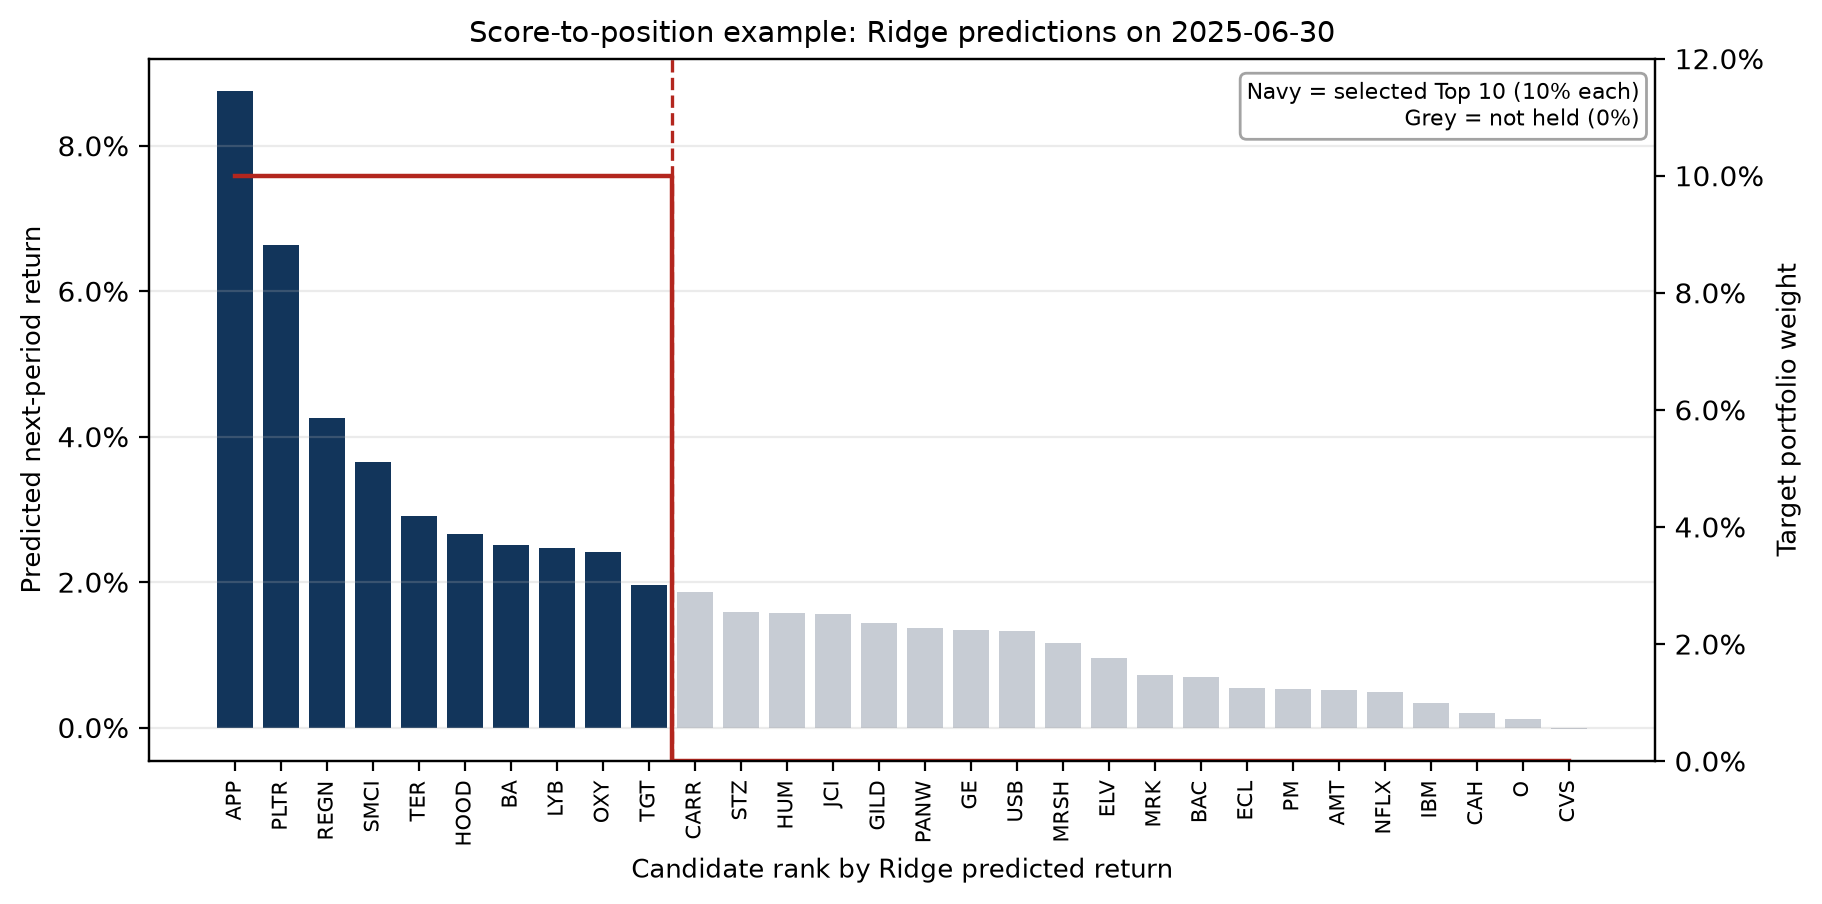
\includegraphics[width=0.90\textwidth]{figures/fig_score_to_position.png}
\caption{Score-to-position example using real Ridge predictions on 30 June 2025. Navy bars are the ten selected stocks, each with a 10\% target weight; grey bars are the twenty candidates with zero target weight.}
\label{fig:score}
\end{figure}

\subsection{Turnover and transaction costs}

Weights drift with realised returns between rebalances. The pre-trade weight of stock $i$ is its post-return weight normalised to sum to one. Turnover is the sum of absolute differences between target and pre-trade weights:
\begin{equation}
\tau_t=\sum_i\left|w_{i,t}-w^{\text{pre}}_{i,t}\right|.
\label{eq:turnover}
\end{equation}
The transaction cost is $\tau_t\times 20$ basis points, and the net return is $R^{\text{net}}_t=R^{\text{gross}}_t-c\tau_t$. Because turnover is a sum of absolute weight changes, both purchases and sales are charged: a 10\% sale and a 10\% purchase each contribute 0.10 to $\tau_t$ and therefore 2 basis points to the cost. Stocks that remain selected are not liquidated and repurchased; only the difference is traded. This is the original convention and is preserved exactly. The automated tests check the first-period cost (1.0 turnover, 0.002 cost), the drift arithmetic and the reconciliation between holdings and portfolio returns.

The 20 basis point assumption is a constant proportional cost. It does not model market impact, bid--ask spread variation, borrow, taxes or capacity. For a monthly strategy holding ten large-cap names it is a reasonable first approximation, but it is not a realistic execution model for a large fund.

\subsection{Cash, constraints and risk}

The portfolio is fully invested. There is no cash buffer, no leverage, no short selling and no explicit risk model. Individual weights are 10\%, so concentration is high by construction. The strategy's beta to SPY is 1.64, which means that a large part of its return is equity-market exposure rather than stock-selection alpha.

\subsection{Distinction from the exploratory extension}

The primary strategy is the 3$\times$3 screen, Ridge Top-10 ranking and equal weights. It is not the same as R1 RidgeWeighted10, which uses momentum selection and prediction-proportional weights capped at 20\%. Section~\ref{sec:extensions} discusses the exploratory strategies separately. Confusing coefficient shrinkage with portfolio allocation is a common error: the $L_2$ penalty stabilises the forecast, while position sizing and caps are separate portfolio decisions.


\section{Out-of-Sample Evaluation}
\label{sec:oos}

\subsection{Protocol and comparability}

The test period is January 2022 to December 2025, covering 48 monthly decision dates. The primary model configuration and its hyperparameters are fixed using training and validation information. All four machine-learning models are refitted on 2010--2021 and evaluated on the same dates; the test period is used once for reporting. The two momentum baselines and the two ETFs are evaluated on the same dates with the same execution convention.

The main experiment and the Ridge extension were produced by different backtest drivers. Before comparing them, the study verifies three things: that both engines use the same 48 decision dates, that SPY and QQQ net returns are identical across engines on every date, and that B3 is the momentum Top-10 of the same thirty-candidate pool used by the main experiment, checked date by date. All three checks pass exactly. The comparison therefore does not mix different return conventions.

Table~\ref{tab:oos} reports the eight strategies. All returns are net of 20 basis points per traded side. Cumulative return is the compounded net return over the 48 months. CAGR is the annualised compound return. Volatility is the annualised standard deviation of monthly net returns. Sharpe and Sortino use a zero risk-free rate and are therefore approximations rather than true excess-return statistics; the definitions follow \citet{sharpe1966} and \citet{sortino1994}. Maximum drawdown is computed from the cumulative wealth series. Turnover is the average monthly sum of absolute weight changes, and cost is the cumulative cost drag in return units.

\begin{table}[H]
\centering
\scriptsize
\begin{tabular}{lrrrrrrrr}
\toprule
Strategy & CAGR & Volatility & Sharpe & Sortino & Max DD & Calmar & Turnover & Cost \\
\midrule
Ridge & 43.0\% & 32.6\% & 1.27 & 2.41 & -28.5\% & 1.51 & 1.26 & 12.07\% \\
LASSO & 42.1\% & 32.3\% & 1.26 & 2.37 & -28.2\% & 1.49 & 1.29 & 12.35\% \\
Random Forest & 40.0\% & 32.8\% & 1.20 & 2.21 & -29.0\% & 1.38 & 1.25 & 12.04\% \\
XGBoost & 38.5\% & 30.8\% & 1.22 & 2.26 & -27.1\% & 1.42 & 1.32 & 12.66\% \\
B1 & 73.1\% & 37.7\% & 1.66 & 3.86 & -19.2\% & 3.81 & 0.65 & 6.24\% \\
B3 & 51.5\% & 29.0\% & 1.59 & 3.68 & -15.0\% & 3.44 & 0.94 & 9.01\% \\
SPY & 12.7\% & 15.3\% & 0.86 & 1.35 & -19.7\% & 0.65 & 0.02 & 0.20\% \\
QQQ & 14.8\% & 19.9\% & 0.80 & 1.25 & -25.6\% & 0.58 & 0.02 & 0.20\% \\
\bottomrule
\end{tabular}
\caption{Out-of-sample performance, 2022--2025 (48 monthly cohorts). All returns are net of 20 basis points per traded side. Sharpe and Sortino use a zero risk-free rate. Turnover is the average monthly sum of absolute weight changes; cost is the cumulative cost drag in return units.}
\label{tab:oos}
\end{table}


\subsection{Four machine-learning models}

Figure~\ref{fig:fourmodel} shows the four ML models under the common trading rule. Ridge has the highest terminal wealth and the highest Sharpe, followed closely by LASSO. Random Forest and XGBoost lag. The ordering is not stable across the whole period: the four curves are close until 2024 and diverge afterwards.

The performance gap is small relative to the uncertainty of a four-year window. Under the original four-model experiment, Ridge's OOS MSE is 0.015057 versus 0.015091 for LASSO, its CAGR is 43.0\% versus 42.1\%, and its Sharpe is 1.27 versus 1.26. These differences are marginal, are not tested for statistical significance, and do not establish universal superiority of Ridge or inferiority of LASSO's sparse selection. The out-of-sample rank IC tells a slightly different story: Random Forest has the highest rank IC at 0.0878, while Ridge is at 0.0619. The ML comparison is therefore best described as inconclusive rather than as a Ridge victory.

\begin{figure}[H]
\centering
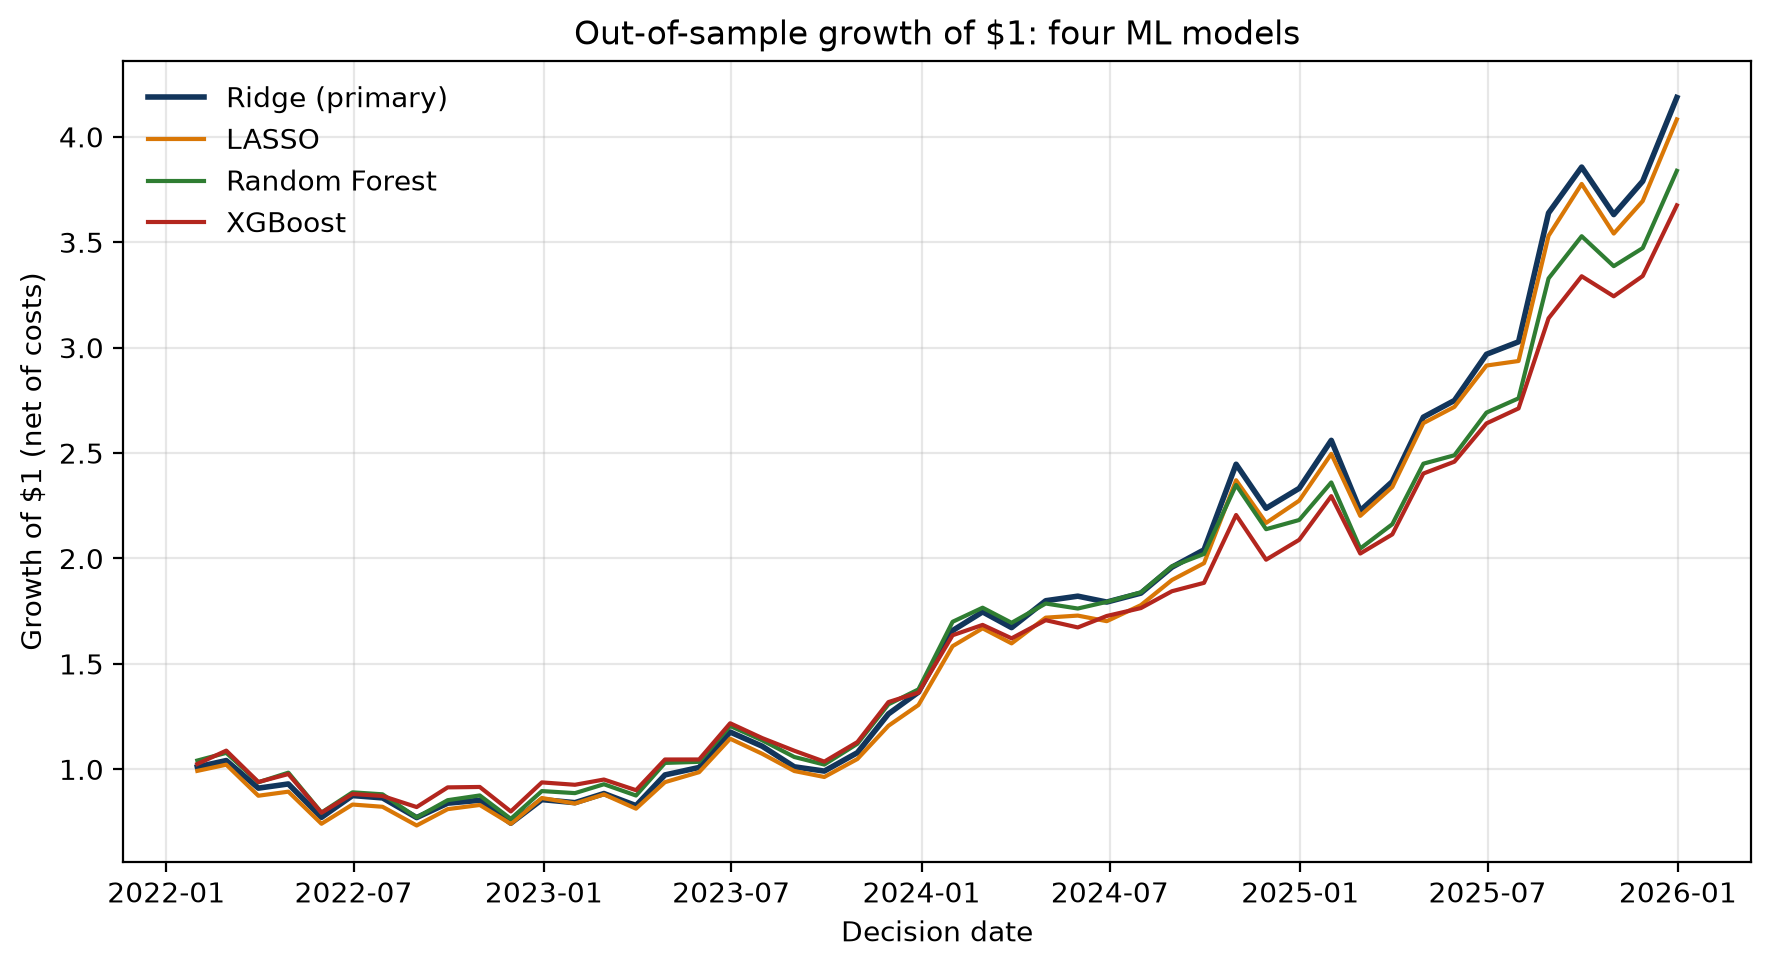
\includegraphics[width=0.60\textwidth]{figures/fig_four_model.png}
\caption{Out-of-sample growth of \$1 for the four machine-learning models under the same Top-10 equal-weight rule. Returns are net of 20 basis points per traded side.}
\label{fig:fourmodel}
\end{figure}

\subsection{Ridge versus momentum baselines and benchmarks}

Figure~\ref{fig:benchmarks} compares the primary Ridge strategy with B1, B3, SPY and QQQ. Ridge compounds to 4.19 times invested capital over the period. SPY compounds to 1.61 and QQQ to 1.74, so the active strategy comfortably beats both investable benchmarks. It does not beat the momentum baselines. B1 compounds to 8.98 and B3 to 5.27.

\begin{figure}[H]
\centering
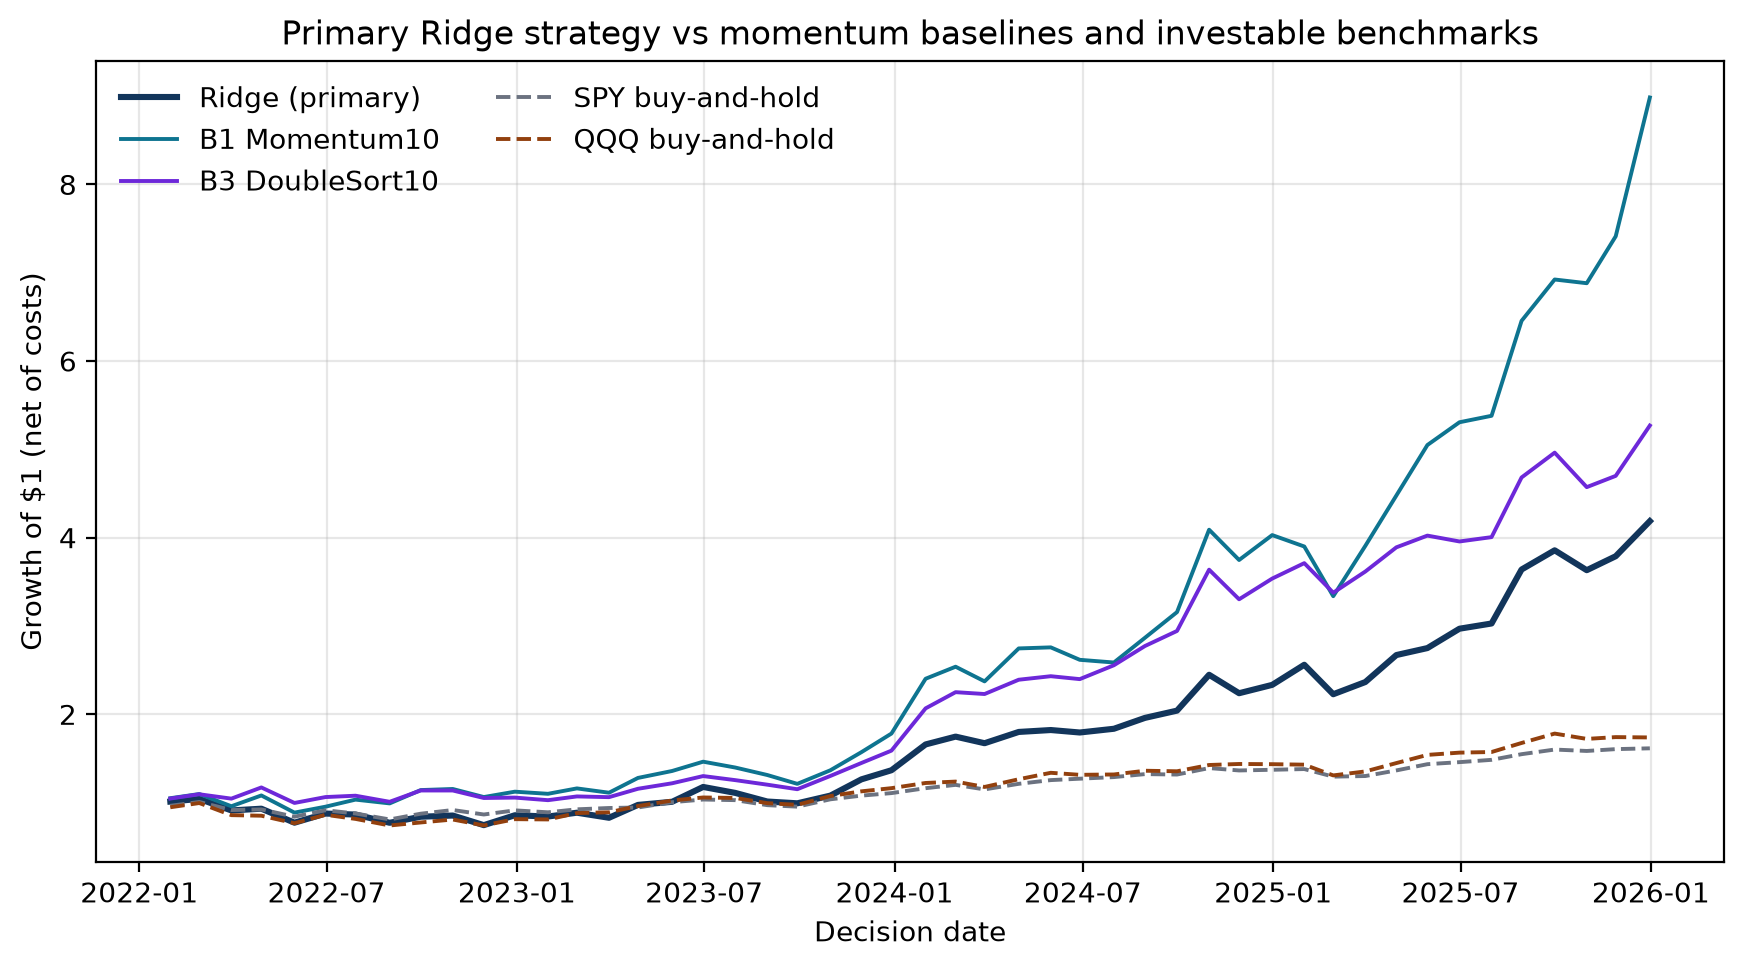
\includegraphics[width=0.60\textwidth]{figures/fig_ridge_benchmarks.png}
\caption{Primary Ridge strategy versus momentum baselines and investable benchmarks, 2022--2025. All series are net of costs.}
\label{fig:benchmarks}
\end{figure}

The numbers in Table~\ref{tab:oos} confirm the visual impression. B1 earns 73.1\% with a 1.66 Sharpe and a -19.2\% maximum drawdown. B3 earns 51.5\% with a 1.59 Sharpe and a -15.0\% drawdown. Ridge earns 43.0\% with a 1.27 Sharpe and a -28.5\% drawdown. Both baselines dominate Ridge on every risk-adjusted dimension, not just on terminal wealth.

The Ridge-versus-B3 comparison is the cleanest evidence on the forecasting question. Both strategies use the same thirty candidates, the same execution and the same costs. The only difference is whether the top ten are chosen by Ridge prediction or by twelve-month momentum. B3's CAGR is 8.5 percentage points higher, its Sharpe is 0.32 higher, and its maximum drawdown is 13.6 percentage points shallower. B3 also trades less: its average monthly turnover is 0.94 versus 1.26 for Ridge. In this sample, the Ridge ranking did not add value over momentum inside the screened pool.

B1's advantage is larger, at 30.1 percentage points of CAGR and 0.39 of Sharpe, but it is not a clean ranking comparison because B1 also selects from the full liquid universe. The difference between B1 and B3 shows how much candidate-universe design matters: expanding the pool from thirty screened names to the full liquid universe and ranking by momentum adds roughly 22 percentage points of CAGR over B3.

\subsection{Eight-strategy summary}

Figure~\ref{fig:summary} and Figure~\ref{fig:risk} summarise the eight strategies. B1 and B3 occupy the top two positions on both CAGR and Sharpe. Ridge is the best of the four ML models but fourth overall. SPY and QQQ are last on CAGR and Sharpe, although their drawdowns are not the worst on every measure. The consistency across CAGR, Sharpe, Sortino, Calmar and drawdown is important: the baseline advantage is not an artefact of one metric.

\begin{figure}[H]
\centering
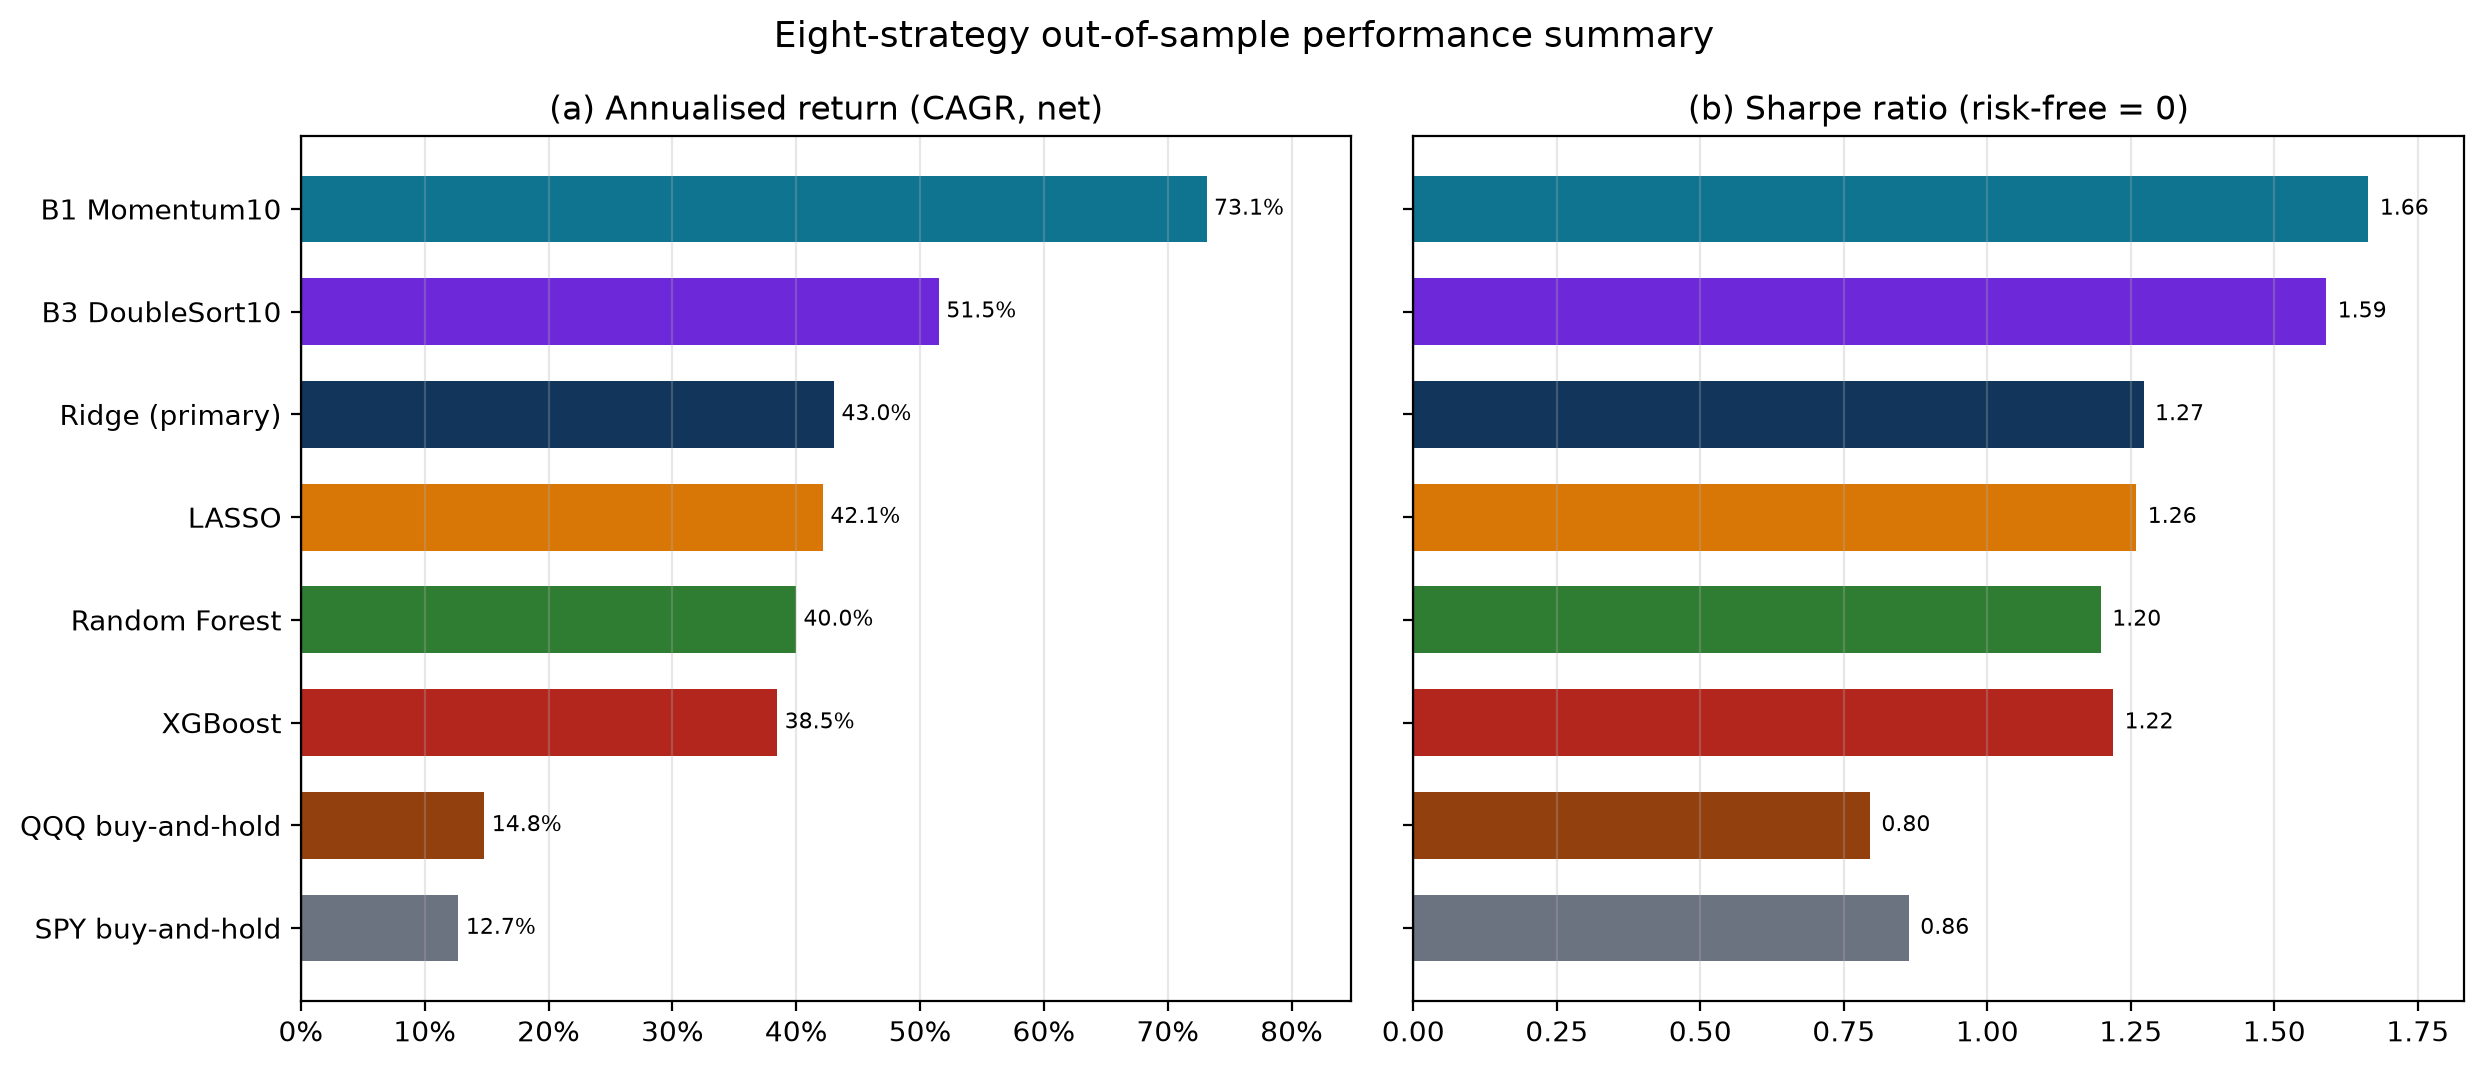
\includegraphics[width=0.66\textwidth]{figures/fig_eight_summary.png}
\caption{Eight-strategy summary: (a) annualised net return and (b) Sharpe ratio. Ridge is the best ML model but ranks behind both momentum baselines.}
\label{fig:summary}
\end{figure}

\subsection{Drawdowns}

Figure~\ref{fig:drawdowns} shows the drawdown paths. Ridge's maximum drawdown of -28.5\% is deeper than B1's -19.2\% and much deeper than B3's -15.0\%. B3 is the most defensive of the active strategies despite having no explicit risk overlay, because its momentum ranking within the screened pool happened to avoid the worst drawdown names in this sample. This should not be interpreted as a structural property of momentum; it is one historical path.

\begin{figure}[H]
\centering
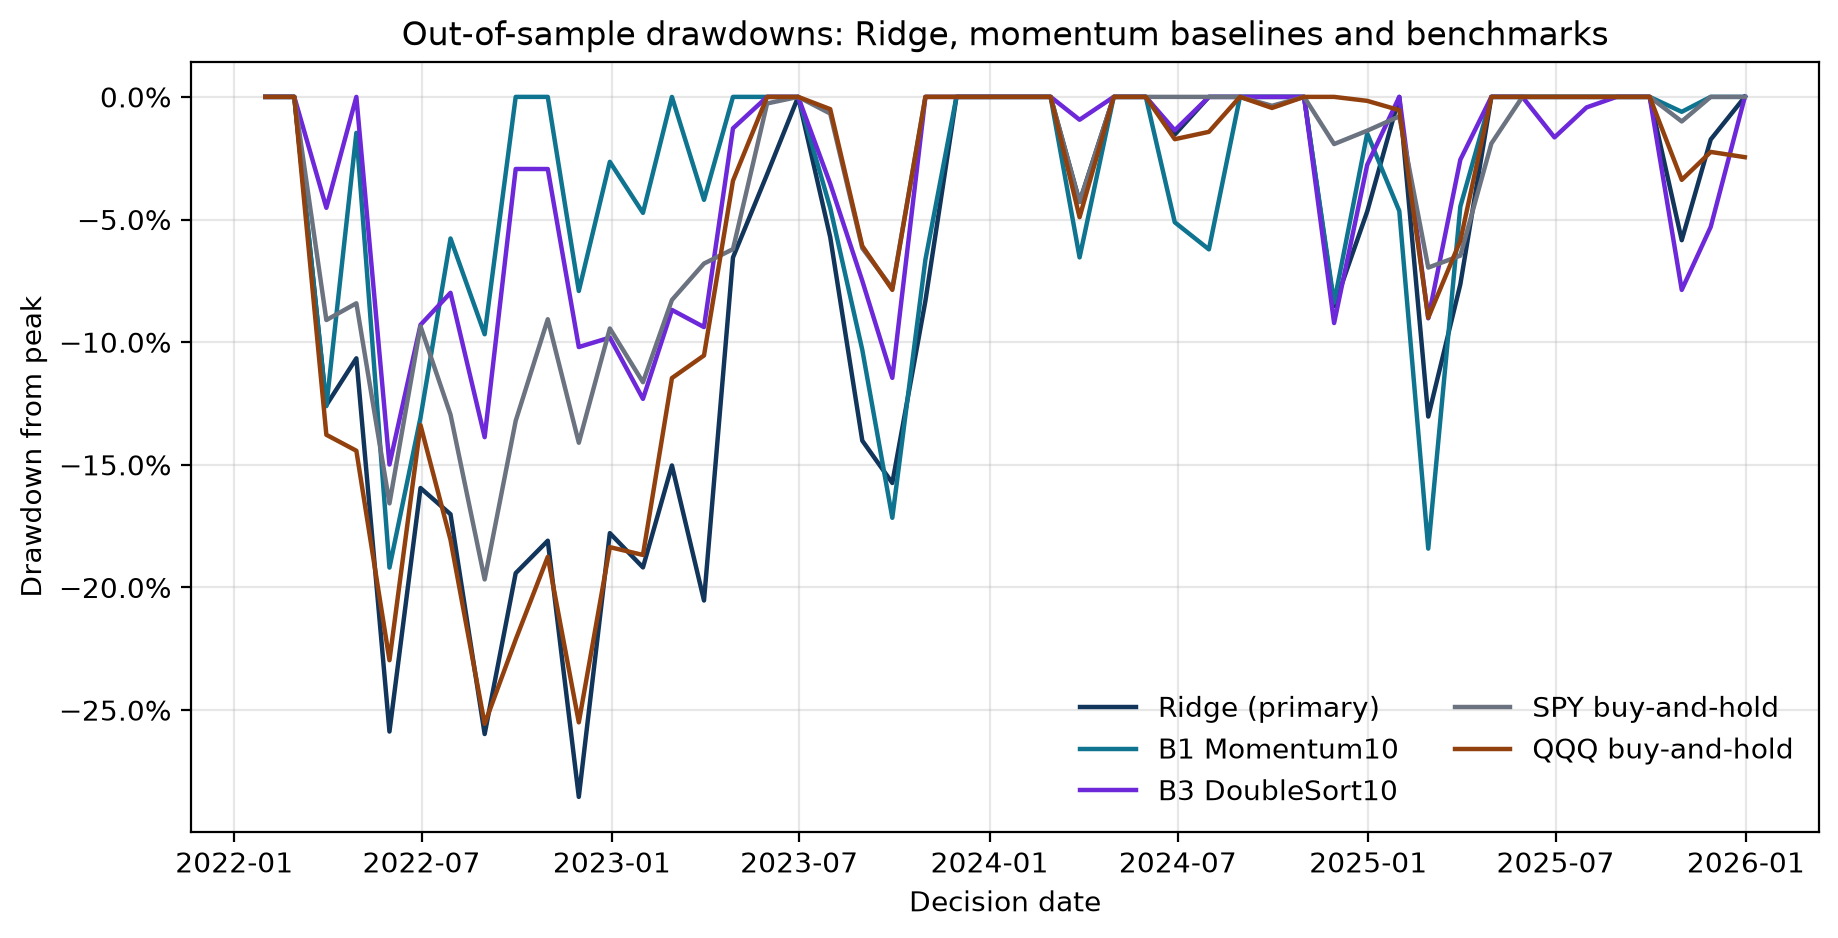
\includegraphics[width=0.60\textwidth]{figures/fig_drawdowns.png}
\caption{Out-of-sample drawdowns for Ridge, B1, B3, SPY and QQQ.}
\label{fig:drawdowns}
\end{figure}

\subsection{Annual returns}

Figure~\ref{fig:annual} and Table~\ref{tab:annual} decompose the performance by calendar year. The baseline advantage is not uniform. In 2022, a down year for equities, Ridge lost 14.4\% while B1 returned 12.3\% and B3 returned 5.6\%. In 2023 Ridge led the baselines slightly, at 59.5\% versus 58.6\% for B1 and 50.3\% for B3. In 2024 B1 and B3 returned 126.1\% and 122.7\% against 70.8\% for Ridge. In 2025 B1 returned 123.0\%, Ridge 79.5\% and B3 49.0\%.

The 2024--2025 gap drives most of the terminal wealth difference. This is consistent with a momentum strategy performing well in a period of strong persistent trends, but the sample is too short to separate a regime effect from a structural advantage. The 2022 result is a reminder that the baselines are not uniformly better: in a declining market, the Ridge portfolio fell while both momentum rules were positive.

\begin{figure}[H]
\centering
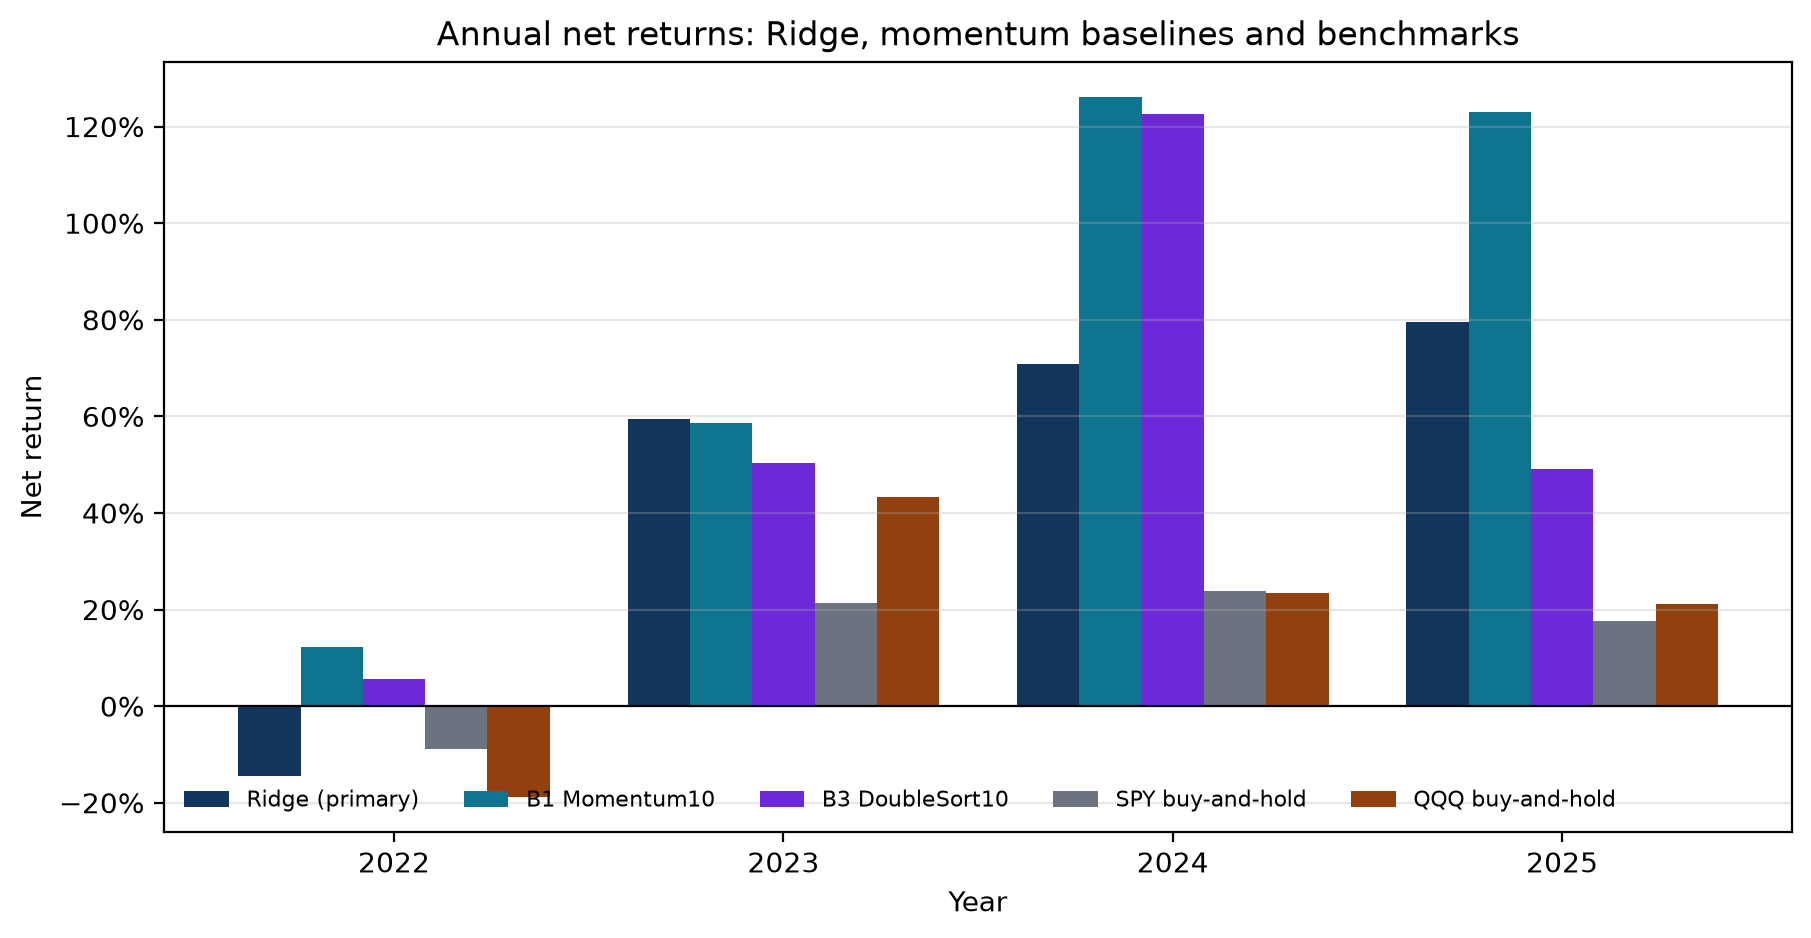
\includegraphics[width=0.60\textwidth]{figures/fig_annual.png}
\caption{Annual net returns for Ridge, B1, B3, SPY and QQQ.}
\label{fig:annual}
\end{figure}

\begin{table}[H]
\centering
\small
\begin{tabular}{lrrrrr}
\toprule
Year & Ridge & B1 & B3 & SPY & QQQ \\
\midrule
2022 & -14.4\% & 12.3\% & 5.6\% & -8.8\% & -18.8\% \\
2023 & 59.5\% & 58.6\% & 50.3\% & 21.4\% & 43.2\% \\
2024 & 70.8\% & 126.1\% & 122.7\% & 23.9\% & 23.3\% \\
2025 & 79.5\% & 123.0\% & 49.0\% & 17.7\% & 21.1\% \\
\bottomrule
\end{tabular}
\caption{Annual net returns. The baseline advantage is not uniform across years: Ridge led in 2023, while B1 and B3 captured much larger returns in 2024.}
\label{tab:annual}
\end{table}


\subsection{Risk-adjusted performance}

Figure~\ref{fig:risk} compares Sharpe ratios and volatilities. Ridge's volatility of 32.6\% is lower than B1's 37.7\% and higher than B3's 29.0\%. The Sharpe ranking is therefore not a simple volatility story: B3 earned a higher return with lower volatility and a shallower drawdown. Ridge's Sharpe of 1.27 is respectable in absolute terms and well above SPY's 0.86, but it is not competitive with B3's 1.59.

\begin{figure}[H]
\centering
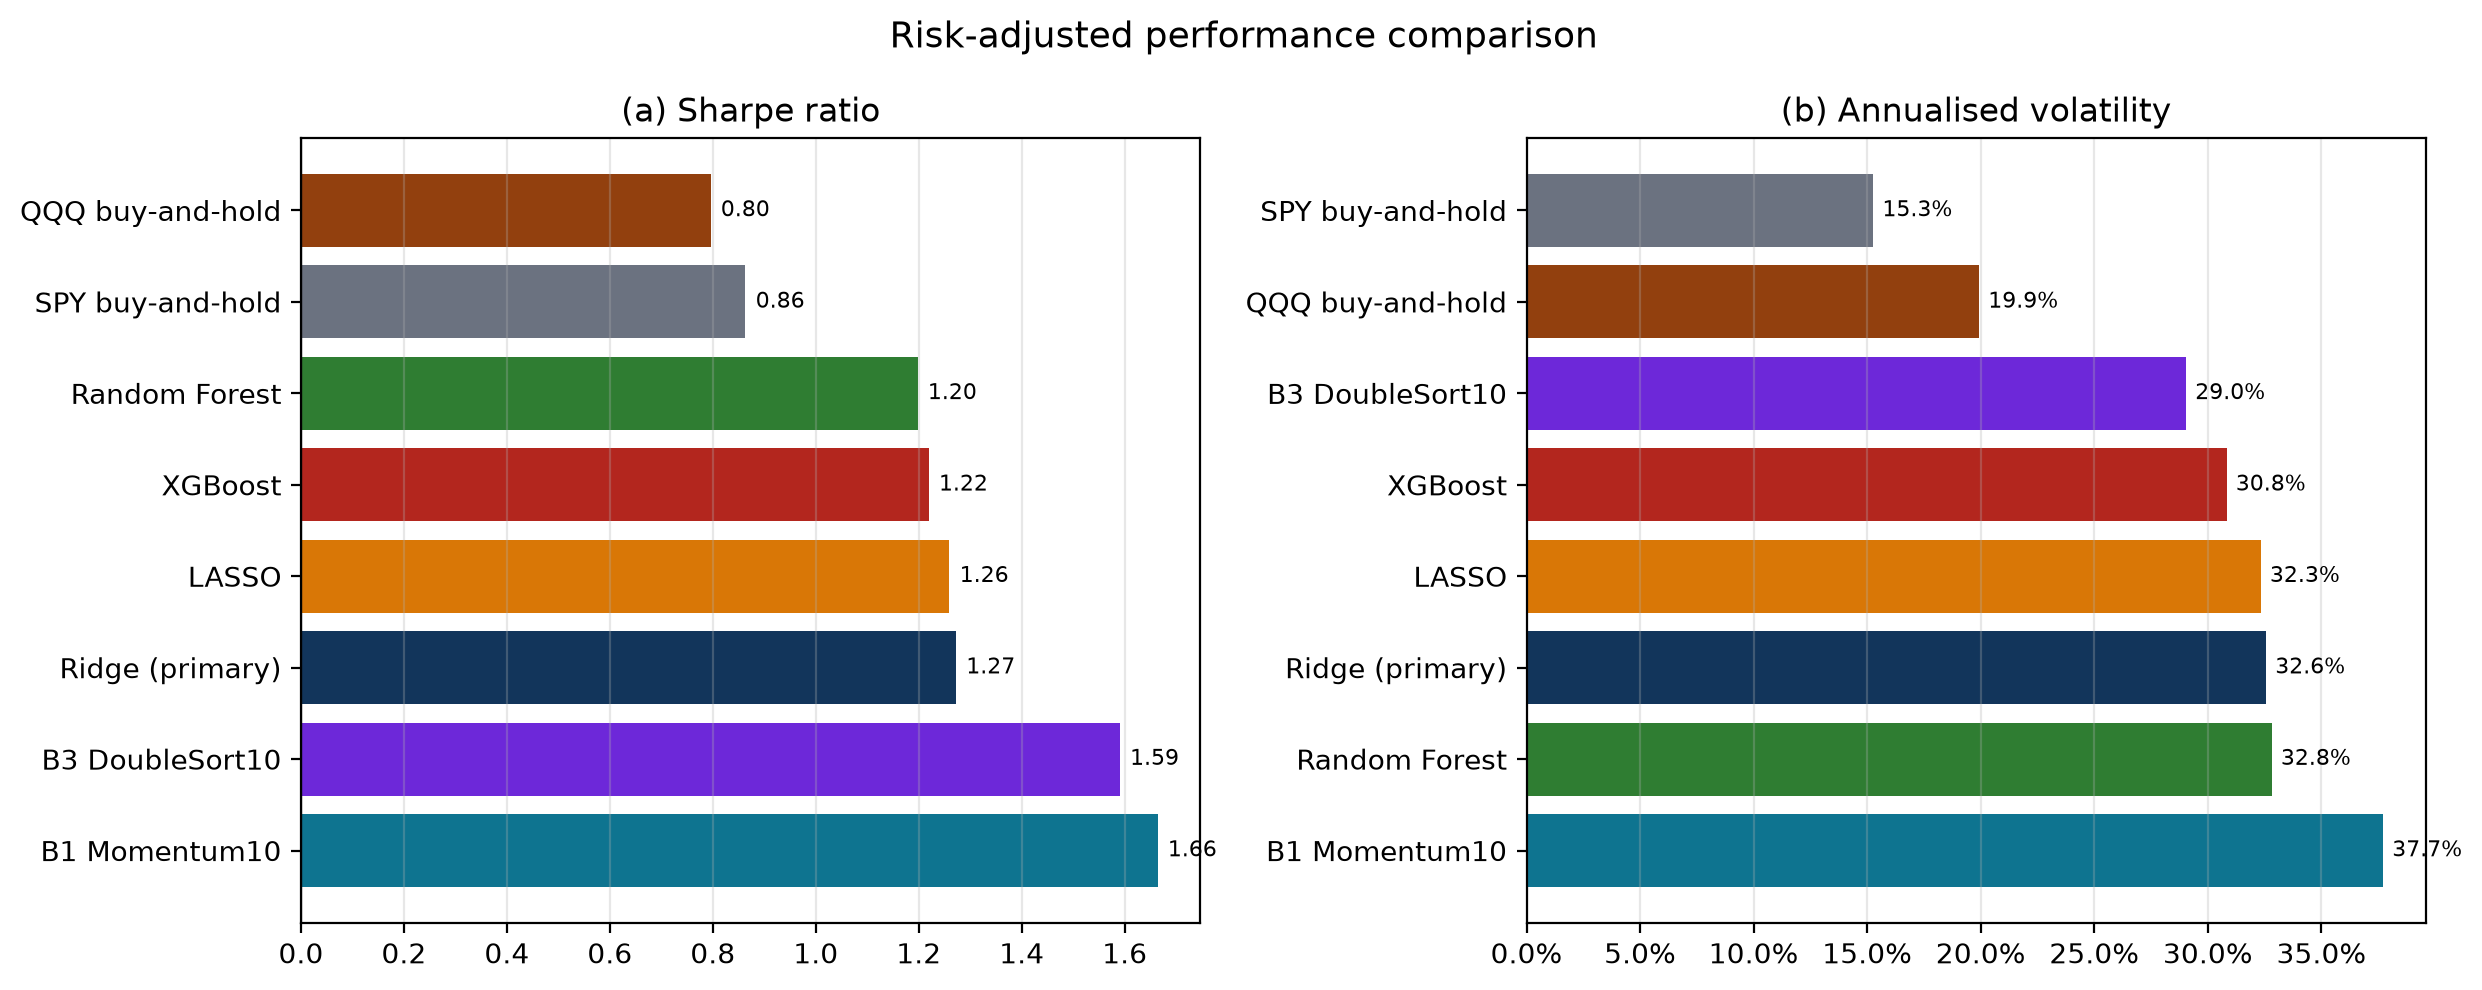
\includegraphics[width=0.66\textwidth]{figures/fig_risk_adjusted.png}
\caption{Risk-adjusted performance: (a) Sharpe ratio and (b) annualised volatility.}
\label{fig:risk}
\end{figure}

\subsection{Prediction performance versus portfolio performance}

The relationship between forecast accuracy and portfolio outcome is weak. Ridge has the lowest OOS MSE and the highest OOS Sharpe among the ML models, but Random Forest has the highest OOS rank IC. LASSO's MSE is almost identical to Ridge's, yet its CAGR is about 0.9 percentage points lower. These differences are small and not statistically distinguishable in a 48-month sample. The more important lesson is that the Top-10 rule uses only the extreme of the ranking; a model that is slightly better on average can be slightly worse at the top of the distribution.

\subsection{Transaction costs and turnover}

Ridge's average monthly turnover is 1.26, compared with 0.65 for B1 and 0.94 for B3. The higher turnover costs 12.07\% of cumulative return over the period, versus 6.24\% for B1 and 9.01\% for B3. Gross of costs, Ridge's CAGR is 47.3\%, so costs reduce its annual return by -4.26 percentage points. The corresponding drag is -2.61 percentage points for B1 and -3.32 for B3. Costs are a material part of the comparison, not a rounding adjustment.

\subsection{Alpha and factor exposure}

Ridge's beta to SPY is 1.64 and its annualised Jensen alpha is 21.7\%, with an information ratio of 1.23. B1's alpha is 49.5\% with a beta of 1.66. The high beta means that a large part of the strategy's return is compensation for market exposure. The alpha is positive and economically meaningful, but it is estimated from 48 monthly observations and is not adjusted for size, value or momentum factors beyond the SPY market factor \citep{fama1993, carhart1997}. It should be read as descriptive, not as a structural estimate of skill.


\section{Interpretation and Economic Discussion}
\label{sec:interpretation}

\subsection{What worked}

Ridge produced a usable cross-sectional ranking. Under the unchanged Top-10 equal-weight rule it earned 43.0\% net compound annual return and a 1.27 Sharpe ratio over 2022--2025, against 12.7\% and 0.86 for SPY and 14.8\% and 0.80 for QQQ. It also produced the highest OOS Sharpe and CAGR among the four forecasting models. The result is not a trivial artefact of market beta alone: the annualised alpha against SPY is 21.7\%, and the information ratio is 1.23.

The validation evidence supports the specification. Ridge has the highest validation rank IC, its coefficient vector moves less between rolling windows than LASSO's, and the correlation structure of the predictors makes a dense shrinkage estimator a reasonable choice. These are genuine arguments in favour of Ridge as a forecasting model.

\subsection{What did not work}

Ridge did not beat simple momentum. B1 and B3 have higher CAGR, higher Sharpe, higher Sortino, higher Calmar and shallower drawdowns. The Ridge-versus-B3 comparison is particularly damaging to the incremental-value claim because it holds the candidate pool, execution and costs fixed. Within that pool, a twelve-month momentum rank produced a better portfolio than the Ridge prediction.

The result is consistent across metrics and across most years, so it is not a single-month anomaly. It is also economically plausible. Twelve-month momentum is a well-documented cross-sectional signal \citep{jegadeesh1993, asness2013}. A regression on fifteen correlated characteristics may dilute that signal with noisier inputs, and the Top-10 selection concentrates the portfolio in the extreme of the predicted distribution, where estimation error is largest.

\subsection{Why simple momentum may outperform a regression}

Three mechanisms can explain the result. First, momentum is a low-dimensional, high-signal characteristic in this universe, while the regression combines fourteen additional predictors whose marginal information may be small. Second, the regression is estimated on a pooled panel with a single coefficient vector, which assumes that the mapping from characteristics to returns is stable across stocks and time. If the mapping is heterogeneous or regime-dependent, the pooled coefficients can be worse than a simple rank. Third, the portfolio selects only ten names; small differences in the middle of the ranking are irrelevant, while errors at the top are costly. A model optimised for average squared error is not necessarily optimised for the top-decile ordering.

\subsection{The importance of candidate-universe design}

B1 and B3 differ only in their candidate universe and ranking implementation, yet B1's CAGR is roughly 22 percentage points higher than B3's. B1 ranks the full liquid universe by momentum, while B3 ranks only the thirty double-sorted candidates. The comparison shows that the screen itself is a powerful filter: the double sort improves the quality of the candidate pool relative to a random subset, but restricting the pool to thirty names also removes high-momentum stocks that the screen did not select. Candidate-universe design is therefore a first-order strategic choice, not a technical detail.

This also means that the Ridge-versus-B1 comparison cannot be interpreted as a pure ranking test. B1 differs in both the pool and the ranking method. Only the Ridge-versus-B3 comparison isolates ranking.

\subsection{Ranking versus weighting}

The extension shows that weighting matters. R1 holds the same stocks as B1 but weights them by Ridge predictions with a 20\% cap. Its CAGR is 87.9\% versus 73.1\% for B1, but its volatility rises from 37.7\% to 44.9\% and its Sharpe is slightly lower (1.64 versus 1.66). The higher absolute return is partly compensation for higher risk and higher turnover. This is a useful reminder that changing the weighting scheme is not the same as improving the forecast, and that a higher CAGR does not by itself indicate a better strategy.

\subsection{Market regimes and the limits of the evidence}

The test period contains very different market environments: a broad decline in 2022, a strong recovery in 2023, and large momentum-driven gains in 2024--2025. The baseline advantage is concentrated in the later years. A four-year window cannot distinguish a structural advantage from a regime effect, and the paper does not claim that momentum will continue to outperform Ridge. The honest conclusion is that the evidence in this sample favours momentum, and that a longer sample or a regime-conditional analysis would be needed to generalise.

\subsection{Limits of the evidence}

The sample is small: 48 monthly observations for the test period, with overlapping one-month holding periods. The strategies are evaluated on a survivorship-biased universe. The cost model is constant and ignores market impact. The models are static during the test period. The primary designation is not a clean pre-registration. These limitations do not invalidate the comparison, but they bound its interpretation. In particular, the paper does not claim statistical significance for the Sharpe differences; it reports them as descriptive evidence from one historical path.


\section{Exploratory Ridge Strategy Extensions}
\label{sec:extensions}

\subsection{Motivation}

The main out-of-sample results motivated a separate question: can Ridge-based portfolio construction be improved by changing the candidate universe, the screening rule, the ranking, the weighting or the diversification constraints? The original exploratory extension addresses this question with six investable sleeves plus SPY and QQQ. The extension is preserved and reported here as exploratory analysis.

\subsection{The extension strategies}

Table~\ref{tab:extension} reports the extension. B1, B2 and B3 are momentum baselines with different universe definitions and portfolio sizes. R1 uses the same stocks as B1 but weights them by Ridge predictions with a 20\% cap. R2 selects the Ridge Top 10 from sixty momentum candidates. R3 imposes a 3/4/3 quota across the high, medium and low momentum groups. SPY and QQQ are buy-and-hold benchmarks.

\begin{table}[H]
\centering
\small
\begin{tabular}{lrrrrrr}
\toprule
Strategy & CAGR & Volatility & Sharpe & Max DD & Turnover & Cost \\
\midrule
B1 Momentum10 & 73.1\% & 37.7\% & 1.66 & -19.2\% & 0.65 & 6.24\% \\
B2 Momentum30 & 31.4\% & 25.9\% & 1.19 & -17.3\% & 0.62 & 5.95\% \\
B3 DoubleSort10 & 51.5\% & 29.0\% & 1.59 & -15.0\% & 0.94 & 9.01\% \\
R1 RidgeWeighted10 & 87.9\% & 44.9\% & 1.64 & -21.5\% & 0.80 & 7.71\% \\
R2 RidgeFree60 & 37.7\% & 39.9\% & 1.01 & -46.6\% & 1.08 & 10.33\% \\
R3 RidgeQuota343 & 22.5\% & 33.3\% & 0.78 & -39.0\% & 1.47 & 14.08\% \\
SPY & 12.7\% & 15.3\% & 0.86 & -19.7\% & 0.02 & 0.20\% \\
QQQ & 14.8\% & 19.9\% & 0.80 & -25.6\% & 0.02 & 0.20\% \\
\bottomrule
\end{tabular}
\caption{Exploratory Ridge extension, 2022--2025. These strategies were designed after earlier out-of-sample results were inspected and therefore do not constitute independent confirmation.}
\label{tab:extension}
\end{table}


\subsection{Results and interpretation}

R1 has the highest CAGR in the extension, at 87.9\%, but its volatility is 44.9\% and its Sharpe is 1.64, slightly below B1's 1.66. The higher return is therefore not a free improvement: it comes with higher risk and higher turnover. R2 earns 37.7\% with a Sharpe of 1.01 and a drawdown of $-$46.6\%, and R3 earns 22.5\% with a Sharpe of 0.78 and a drawdown of $-$39.0\%. Both are weaker than B3's 51.5\%, 1.59 and $-$15.0\%.

The extension illustrates three points. First, prediction-based weighting can increase absolute return while leaving risk-adjusted performance roughly unchanged or worse. Second, changing the candidate universe or the Ridge training sample changes the fitted model and can change the result even when the economic rule is similar; the training universe is part of the model specification. Third, diversification constraints such as the 3/4/3 quota can reduce concentration but do not necessarily improve performance.

\subsection{Status of the extension}

These analyses are exploratory. Their design was informed by previously viewed out-of-sample results, so they do not provide fresh independent confirmation. They are reported for economic insight, not as replacements for the primary strategy. The primary Ridge strategy remains the 3$\times$3 screen, Ridge Top-10 ranking and equal-weight rule, regardless of whether an extension earned a higher CAGR.


\section{Limitations and Future Research}
\label{sec:limitations}

\subsection{Data limitations}

Using current S\&P 500 constituents to construct the historical equity universe introduces potential survivorship and constituent-selection bias into the active stock-selection strategies. Firms that were removed from the index are absent and current survivors are over-represented, which may overstate the active strategies' historical performance relative to SPY and QQQ. The buy-and-hold benchmark returns are calculated directly from historical ETF prices and are not affected by the same constituent-selection mechanism. Data-vendor price adjustments and corporate-action treatment can affect both individual-stock histories and ETF return calculations. The direction or magnitude of the survivorship effect is not precisely measured here, and a point-in-time constituent database would be required to correct it.

Vendor data also introduce limitations. Yahoo Finance adjusted prices can be revised, and the snapshot is not an exchange-grade point-in-time record. The data are adequate for an academic exercise but not for production research.

\subsection{Statistical limitations}

The test period contains 48 monthly observations. Monthly returns are overlapping in the sense that the holding period spans the decision interval, and the strategies share the same candidate pool, so the effective number of independent observations is smaller than 48. The Sharpe differences reported here are not accompanied by confidence intervals or multiple-testing corrections. A block bootstrap or a deflated Sharpe ratio \citep{bailey2014} would provide a more formal assessment, but with four years of data the power would remain low.

\subsection{Model uncertainty}

The comparison evaluates four algorithms and twenty-three configurations. Model uncertainty is therefore not fully captured by the selected configuration: a different but equally plausible configuration could produce different results. The paper mitigates this by using a small pre-declared grid and by reporting the full validation table, but it does not perform a full model-averaging exercise.

\subsection{Transaction-cost assumptions}

The 20 basis point cost is constant and proportional. It does not model market impact, spread variation, borrow costs, taxes or capacity. For a ten-stock large-cap portfolio the assumption is reasonable, but a larger portfolio would face higher impact costs. The cost sensitivity of the results is not explored beyond the gross-versus-net comparison reported in Section~\ref{sec:oos}.

\subsection{Market-regime sensitivity}

The baseline advantage is concentrated in 2024--2025. A longer sample or a regime-conditional analysis would be needed to determine whether the result is structural or cyclical. The paper does not claim that momentum will continue to outperform Ridge.

\subsection{Test-informed exploratory analysis}

The exploratory extension was designed after earlier out-of-sample results were inspected. It is therefore not an independent confirmation of any hypothesis. The paper labels it exploratory and does not use it to select the primary strategy.

\subsection{Future research}

Four extensions would strengthen the analysis. First, a point-in-time constituent database would remove survivorship bias. Second, rolling out-of-sample retraining with a fixed window would test whether the static model is the limiting factor. Third, a regime-conditional analysis would test whether Ridge adds value in specific market states. Fourth, a formal multiple-testing framework would quantify the uncertainty around the Sharpe differences. None of these extensions is claimed in this paper.


\section{Conclusion}
\label{sec:conclusion}

The paper asked whether Ridge Regression, trained on economically motivated predictors, can generate useful cross-sectional rankings and improve a systematic equity portfolio relative to simpler alternatives. The answer is nuanced.

Ridge works as a forecasting model. It produces a usable ranking, earns 43.0\% net CAGR and a 1.27 Sharpe over 2022--2025, and beats SPY and QQQ by a wide margin after costs. It also has the highest OOS Sharpe and CAGR among the four machine-learning models, and its validation rank IC is the highest of the four. The Ridge specification is supported by the correlation structure of the predictors and by rolling coefficient-stability diagnostics: its coefficients move about 37.4\% less between windows than LASSO's, even though it sign-flips more often.

Ridge does not beat simple momentum. B1 earns 73.1\% with a 1.66 Sharpe, and B3 earns 51.5\% with a 1.59 Sharpe and a -15.0\% drawdown. Within the same candidate pool, the Ridge ranking underperforms a momentum ranking by 8.5 percentage points of CAGR and 0.32 of Sharpe, with higher turnover. The result is consistent across CAGR, Sharpe, Sortino, Calmar and drawdown, and it is not driven by a single year.

The economic lesson is that a statistically sensible forecasting model is not automatically a better portfolio rule. Momentum is a low-dimensional, high-signal characteristic in this universe, and the Top-10 portfolio concentrates on the extreme of the ranking, where estimation error is largest. Candidate-universe design is at least as important as the forecasting algorithm: B1's broader universe contributes roughly 22 percentage points of CAGR relative to B3, independent of the model.

The paper is transparent about its limitations. The universe is survivorship-biased, the test window is short, the cost model is simple, and the Ridge designation is not a clean pre-registration because the project history includes prior out-of-sample review. These limitations do not overturn the comparison, but they bound its interpretation. The defensible conclusion is that Ridge is an economically motivated model that adds value relative to passive benchmarks but does not establish incremental value over momentum-based selection in this sample. Reporting that result, rather than selecting a different strategy after seeing the test period, is the main contribution of the exercise.


\section{Reproducibility and AI-Use Declaration}
\label{sec:reproducibility}

\subsection{Project structure and commands}

The repository contains \texttt{src/} for source code, \texttt{config/} for the experiment configuration, \texttt{tests/} for the automated suite, \texttt{results/} for generated tables and figures, \texttt{report/} for this document and its LaTeX source, and \texttt{notebooks/} for the executed notebook.

The complete pipeline is reproduced with:
\begin{verbatim}
python run_pipeline.py --stage validation
python run_pipeline.py --stage designate --approve
python run_pipeline.py --stage refit
python run_pipeline.py --stage oos
python run_pipeline.py --stage extension
python run_pipeline.py --stage eight
python run_tests.py --notebook
\end{verbatim}
The report is rebuilt with \texttt{python report/build\_report.py}. The environment is Python 3.11.4 with numpy 1.26.4, pandas 2.2.3, scikit-learn 1.9.1, XGBoost 3.2.0, matplotlib 3.11.2 and PyYAML 6.0. The random seed is 42.

\subsection{Outputs and audit trail}

Validation tables and fifteen figures are under \texttt{results/validation/}. Out-of-sample tables and Figures~2--7 are under \texttt{results/oos/} and \texttt{results/oos/eight\_strategy/}. The exploratory extension is under \texttt{results/extensions/}. The correlation and coefficient-stability diagnostics are under \texttt{results/diagnostics/}. Serialized models are under \texttt{results/models/refit/}.

The primary-model contract is \texttt{results/validation/primary\_model\_contract.json}. It records the primary model, its hyperparameters, the validation metrics, the diagnostic evidence, the historical LASSO audit and the chronology disclosure. The historical LASSO selection contract is archived under \texttt{results/validation/archive/} and is not overwritten.

\subsection{AI-use declaration}

This revision was prepared with AI assistance (DeepSeek Harness) for code restructuring, test generation, diagnostic integration, figure production and LaTeX drafting. All numerical results were produced by executing the repository code on the historical data snapshot. The original strategy, data pipeline and exploratory extension were authored by the project team. The AI assistant did not have access to any data beyond the supplied project files, and no result was fabricated or manually inserted.

\subsection{Chronology disclosure}

The original project pre-specified Ridge. A later engineering revision introduced an automatic minimum-MSE rule that selected LASSO, and out-of-sample results were reviewed during that revision. The Ridge designation was restored afterwards on economic and diagnostic grounds. The primary-model contract records that the designation is not a clean pre-registration and that it was informed by prior out-of-sample review. No test-period metric was used to choose Ridge or its $\alpha$, but the designation should not be presented as a blind pre-registration.

\begin{thebibliography}{99}
\small
\setlength{\itemsep}{1pt}

\bibitem[Asness et al.(2013)]{asness2013}
Asness, C. S., Moskowitz, T. J., and Pedersen, L. H. (2013).
Value and momentum everywhere.
\textit{Journal of Finance}, 68(3), 929--985.

\bibitem[Bailey and L\'opez de Prado(2014)]{bailey2014}
Bailey, D. H., and L\'opez de Prado, M. (2014).
The deflated Sharpe ratio: correcting for selection bias, backtest overfitting, and non-normality.
\textit{Journal of Portfolio Management}, 40(5), 94--107.

\bibitem[Breiman(2001)]{breiman2001}
Breiman, L. (2001).
Random forests.
\textit{Machine Learning}, 45(1), 5--32.

\bibitem[Campbell and Thompson(2008)]{campbell2008}
Campbell, J. Y., and Thompson, S. B. (2008).
Predicting excess stock returns out of sample: can anything beat the historical average?
\textit{Review of Financial Studies}, 21(4), 1509--1531.

\bibitem[Carhart(1997)]{carhart1997}
Carhart, M. M. (1997).
On persistence in mutual fund performance.
\textit{Journal of Finance}, 52(1), 57--84.

\bibitem[Chen and Guestrin(2016)]{chen2016}
Chen, T., and Guestrin, C. (2016).
XGBoost: a scalable tree boosting system.
In \textit{Proceedings of the 22nd ACM SIGKDD International Conference on Knowledge Discovery and Data Mining}, 785--794.

\bibitem[Fama and French(1993)]{fama1993}
Fama, E. F., and French, K. R. (1993).
Common risk factors in the returns on stocks and bonds.
\textit{Journal of Financial Economics}, 33(1), 3--56.

\bibitem[Feng et al.(2020)]{feng2020}
Feng, G., Giglio, S., and Xiu, D. (2020).
Taming the factor zoo: a test of new factors.
\textit{Journal of Finance}, 75(3), 1327--1370.

\bibitem[Freyberger et al.(2020)]{freyberger2020}
Freyberger, J., Neuhierl, A., and Weber, M. (2020).
Dissecting characteristics nonparametrically.
\textit{Review of Financial Studies}, 33(5), 2326--2377.

\bibitem[Gu et al.(2020)]{gu2020}
Gu, S., Kelly, B., and Xiu, D. (2020).
Empirical asset pricing via machine learning.
\textit{Review of Financial Studies}, 33(5), 2223--2273.

\bibitem[Hoerl and Kennard(1970)]{hoerl1970}
Hoerl, A. E., and Kennard, R. W. (1970).
Ridge regression: biased estimation for nonorthogonal problems.
\textit{Technometrics}, 12(1), 55--67.

\bibitem[Hou et al.(2020)]{hou2020}
Hou, K., Xue, C., and Zhang, L. (2020).
Replicating anomalies.
\textit{Review of Financial Studies}, 33(5), 2019--2133.

\bibitem[Jegadeesh(1990)]{jegadeesh1990}
Jegadeesh, N. (1990).
Evidence of predictable behavior of security returns.
\textit{Journal of Finance}, 45(3), 881--898.

\bibitem[Jegadeesh and Titman(1993)]{jegadeesh1993}
Jegadeesh, N., and Titman, S. (1993).
Returns to buying winners and selling losers: implications for stock market efficiency.
\textit{Journal of Finance}, 48(1), 65--91.

\bibitem[Kelly et al.(2019)]{kelly2019}
Kelly, B. T., Pruitt, S., and Su, Y. (2019).
Characteristics are covariances: a unified model of risk and return.
\textit{Journal of Financial Economics}, 134(3), 501--524.

\bibitem[McLean and Pontiff(2016)]{mclean2016}
McLean, R. D., and Pontiff, J. (2016).
Does academic research destroy stock return predictability?
\textit{Journal of Finance}, 71(1), 5--32.

\bibitem[Moskowitz et al.(2012)]{moskowitz2012}
Moskowitz, T. J., Ooi, Y. H., and Pedersen, L. H. (2012).
Time series momentum.
\textit{Journal of Financial Economics}, 104(2), 228--250.

\bibitem[Sharpe(1966)]{sharpe1966}
Sharpe, W. F. (1966).
Mutual fund performance.
\textit{Journal of Business}, 39(1), 119--138.

\bibitem[Sortino and Price(1994)]{sortino1994}
Sortino, F. A., and Price, L. N. (1994).
Performance measurement in a downside risk framework.
\textit{Journal of Investing}, 3(3), 59--64.

\bibitem[Tibshirani(1996)]{tibshirani1996}
Tibshirani, R. (1996).
Regression shrinkage and selection via the lasso.
\textit{Journal of the Royal Statistical Society: Series B}, 58(1), 267--288.

\end{thebibliography}

\appendix
\section{Diagnostic Figures}
\label{app:diagnostics}
\setcounter{figure}{0}
\renewcommand{\thefigure}{A\arabic{figure}}

The two figures below support the model-justification discussion in Section~\ref{sec:model}. They are placed in the appendix as Figures~A1--A2 so that the main text keeps the score-to-position and out-of-sample exhibits in sequence.

\begin{figure}[H]
\centering
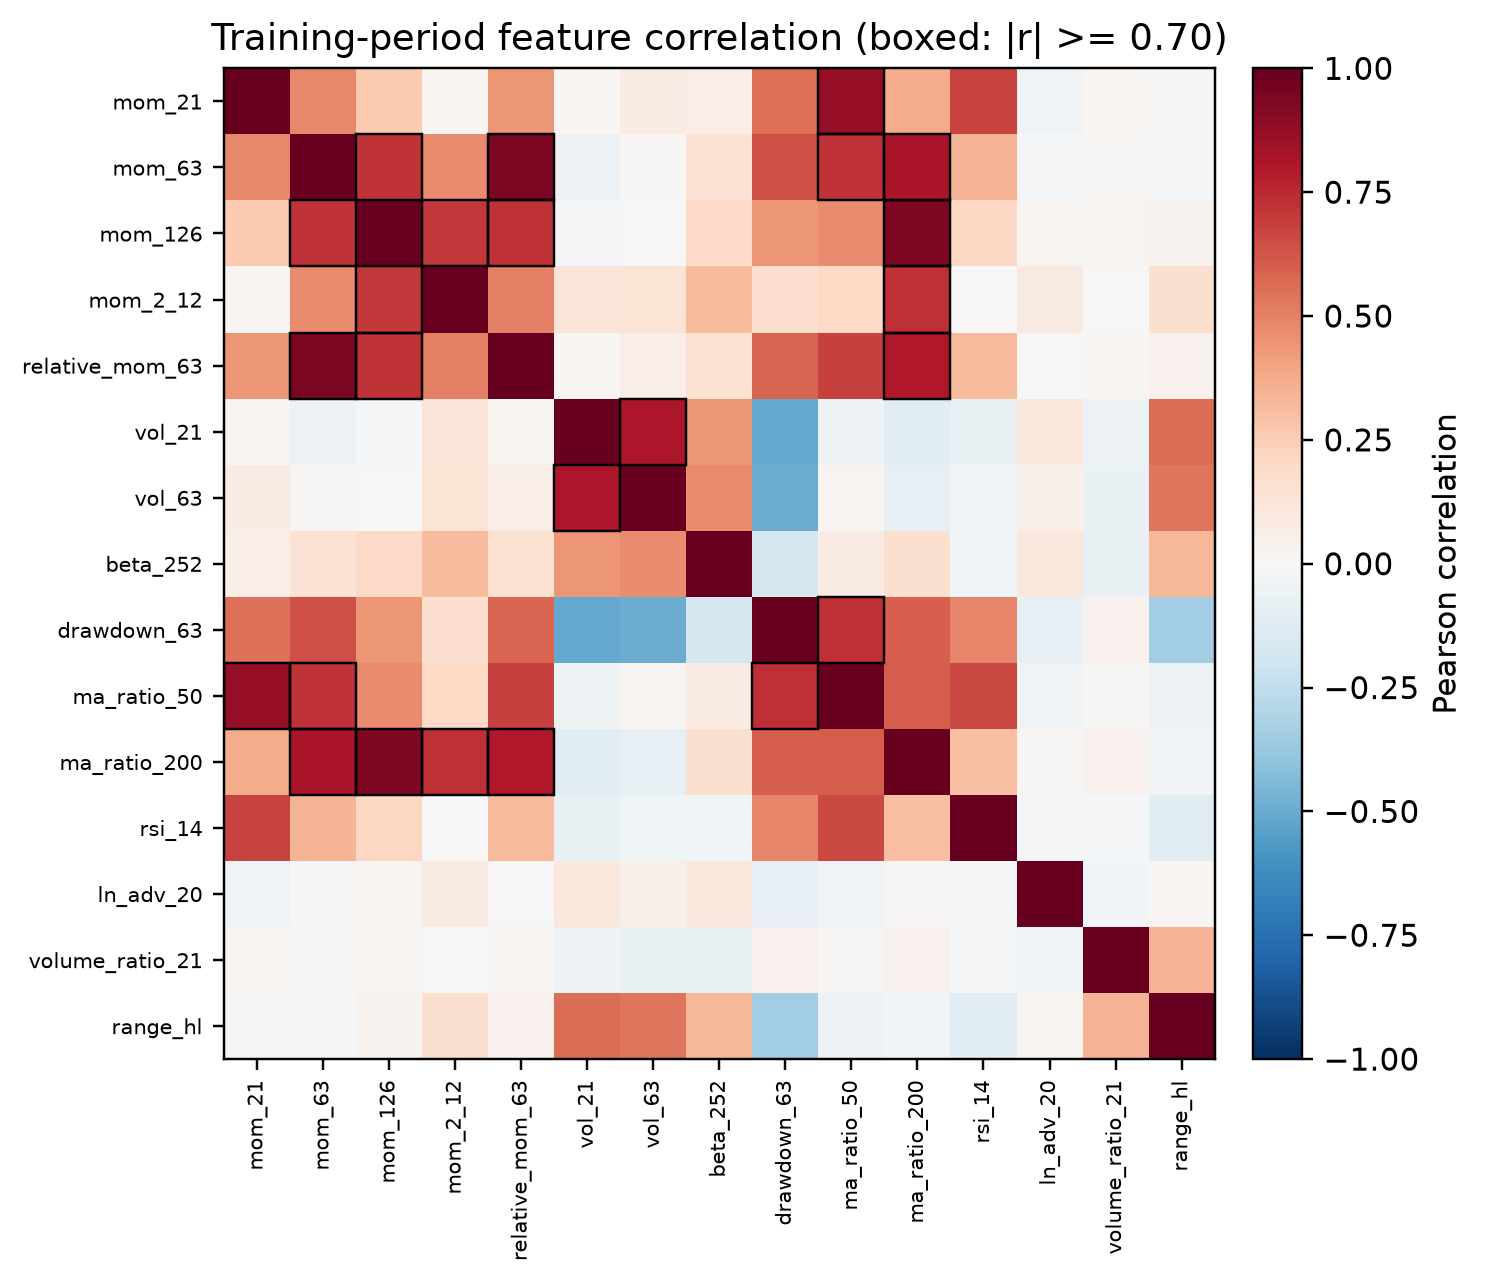
\includegraphics[width=0.55\textwidth]{figures/fig_correlation.png}
\caption{Training-period Pearson correlation matrix of the fifteen features. Boxed cells have absolute correlation of at least 0.70.}
\label{fig:corr}
\end{figure}

\begin{figure}[H]
\centering
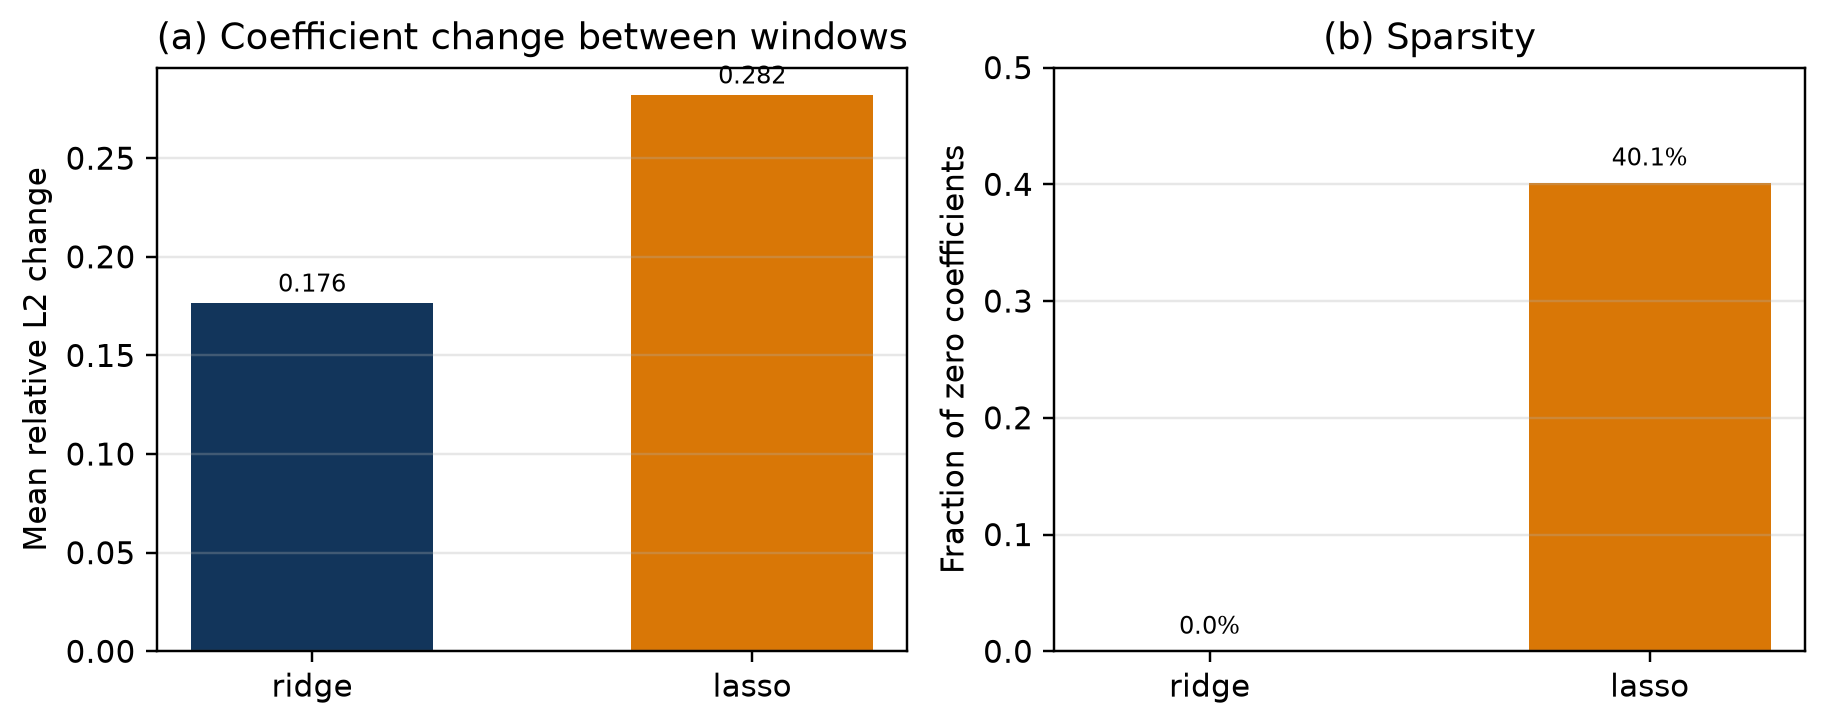
\includegraphics[width=0.60\textwidth]{figures/fig_stability.png}
\caption{Rolling-window coefficient stability. Panel (a) shows the distribution of relative $L_2$ coefficient changes between adjacent 60-month windows; panel (b) shows the fraction of zero coefficients. Ridge changes less on average but sign-flips more often.}
\label{fig:stability}
\end{figure}

\section{Supplementary Tables}

Table~\ref{tab:gross_net} reports the gross-to-net decomposition and market-factor exposure for the eight strategies, complementing the net figures in Table~\ref{tab:oos}.

\begin{table}[H]
\centering
\small
\begin{tabular}{lrrrrr}
\toprule
Strategy & Gross CAGR & Net CAGR & Cost drag (pp) & Beta & Alpha \\
\midrule
Ridge & 47.30\% & 43.04\% & 4.26 & 1.64 & 21.73\% \\
LASSO & 46.49\% & 42.15\% & 4.34 & 1.66 & 20.54\% \\
Random Forest & 44.14\% & 39.98\% & 4.17 & 1.62 & 19.46\% \\
XGBoost & 42.80\% & 38.46\% & 4.35 & 1.50 & 19.27\% \\
B1 & 75.74\% & 73.13\% & 2.61 & 1.66 & 49.50\% \\
B3 & 54.83\% & 51.51\% & 3.32 & 1.28 & 33.58\% \\
SPY & 12.78\% & 12.72\% & 0.06 & 1.00 & 0.00\% \\
QQQ & 14.87\% & 14.81\% & 0.06 & 1.22 & -0.21\% \\
\bottomrule
\end{tabular}
\caption{Gross-versus-net decomposition and market-factor exposure. Cost drag is the difference between gross and net CAGR in percentage points. Alpha is annualised Jensen alpha against SPY with a zero risk-free rate.}
\label{tab:gross_net}
\end{table}





\end{document}
